%%
%% Copyright 2007, 2008, 2009 Elsevier Ltd
%%
%% This file is part of the 'Elsarticle Bundle'.
%% ---------------------------------------------
%%
%% It may be distributed under the conditions of the LaTeX Project Public
%% License, either version 1.2 of this license or (at your option) any
%% later version.  The latest version of this license is in
%%    http://www.latex-project.org/lppl.txt
%% and version 1.2 or later is part of all distributions of LaTeX
%% version 1999/12/01 or later.
%%
%% The list of all files belonging to the 'Elsarticle Bundle' is
%% given in the file `manifest.txt'.
%%

%% Template article for Elsevier's document class `elsarticle'
%% with numbered style bibliographic references
%% SP 2008/03/01

\documentclass[preprint,12pt]{elsarticle}

\usepackage{amssymb, amsmath}
\usepackage[utf8]{inputenc}
\usepackage{tabularx}
\usepackage{enumerate}
\usepackage{dsfont}
\usepackage{graphicx}
\usepackage{color}
\usepackage{multicol}

%% The amsthm package provides extended theorem environments
%% \usepackage{amsthm}

%% The lineno packages adds line numbers. Start line numbering with
%% \begin{linenumbers}, end it with \end{linenumbers}. Or switch it on
%% for the whole article with \linenumbers.
%% \usepackage{lineno}

\journal{Journal of Theoretical Biology}

\begin{document}

\renewcommand{\thefootnote}{$*$}

\begin{frontmatter}

%% Title, authors and addresses

%% use the tnoteref command within \title for footnotes;
%% use the tnotetext command for theassociated footnote;
%% use the fnref command within \author or \address for footnotes;
%% use the fntext command for theassociated footnote;
%% use the corref command within \author for corresponding author footnotes;
%% use the cortext command for theassociated footnote;
%% use the ead command for the email address,
%% and the form \ead[url] for the home page:
%% \title{Title\tnoteref{label1}}
%% \tnotetext[label1]{}
%% \author{Name\corref{cor1}\fnref{label2}}
%% \ead{email address}
%% \ead[url]{home page}
%% \fntext[label2]{}
%% \cortext[cor1]{}
%% \address{Address\fnref{label3}}
%% \fntext[label3]{}

\title{On the reinfection of individuals in stochastic epidemic models}

%% use optional labels to link authors explicitly to addresses:
%% \author[label1,label2]{}
%% \address[label1]{}
%% \address[label2]{}

\author{M. L\'opez-Garc\'ia$^{a,}\footnote{Corresponding author: m.lopezgarcia@leeds.ac.uk}$, A. Camacho$^{b,c}$}

\address{$^a${\it Department of Applied Mathematics, School of Mathematics, University of Leeds, LS2 9JT Leeds, UK}\\
$^b${\it London School of Hygiene and Tropical Medicine,  WC1E 7HT London, UK}\\
$^c${\it Epicentre, Medecins Sans Frontieres, 55 Rue Crozatier 75012 Paris, France}}

\begin{abstract}
Our interest in this paper is on a number of epidemic models that allow for reinfection of individuals among a closed well-mixed finite population.
For stochastic versions of a number of SIS- and SIR-type epidemic models, that account for partial, temporary or no immunity, allowing then for reinfection of individuals, we analytically quantify a main summary statistic: the probability that a given individual suffers exactly $M$ infections during the epidemic, for any value $M\geq0$. Our analysis has the particular feature that
allows to study specific individuals that might behave differently against the disease than the rest of individuals in the population ({\it i.e.}, to consider that the individual under study has different infectivity, susceptibility or ability to recover). We illustrate our analysis by means of... and explain how this summary statistic relates to another important concept in mathematical epidemiology, {\it epidemic fade-out}.
\end{abstract}

\begin{keyword}
continuous-time Markov chain; SIS; SIRS; reinfection; epidemic fade-out;
\end{keyword}

\end{frontmatter}

\section{Introduction}
\label{Sect1}

\par Mathematical epidemiological models have been extensively studied and used in the literature for analysing disease spread dynamics. Depending on the disease under study and the population of
individuals among which this disease spreads, different models have been proposed: the $SIS$ epidemic model where individuals are infected and become susceptible immediately after recovery; the $SIR$ model in which after individuals recover they gain immunity against the disease, which lasts forever (this {\it recovery} might also mean {\it removal}, representing that individuals die or leave the system not playing a role any more in the disease spread dynamics); the $SEIR$ epidemic model where a latent infection period is considered in which individuals are infected but not infectious; or the $SIRS$ epidemic model where immune individuals recover susceptibility after a period of time.

\par A wide range of variants to these models have been proposed in order to account for specific characteristics of the disease under study or the population being affected. Stochastic models
have usually been considered specially when analysing small populations ({\it e.g.,} hospital wards \cite{artalejo2011sis,lopez2016stochastic}, prisons \cite{hotta2010bayesian}, schools \cite{artalejo2010number,stone2008stochastic} or families \cite{economou2015stochastic}), while deterministic counterparts have been developed for large populations \cite{allen2000comparison}. Compartmental models assume that individuals within the population under study are homogeneous in terms of their behaviour against the disease ({\it i.e.,} equal infectivity, susceptibility and ability to recover), an assumption that simplifies the mathematical analysis and the estimation of parameters in the model. Heterogeneous populations can be considered instead by means of increasing the number of compartments in the model ({\it e.g.,} analysing populations structured in households \cite{ball2016reproduction,pellis2012reproduction}) or, as the extreme case, by developing agent-based models where the epidemic dynamics of each specific individual in the population are tracked \cite{graw2012agent}. The analysis of agent-based models from a stochastic perspective usually leads to the analysis of continuous-time Markov chains on networks \cite{economou2015stochastic,lopez2016stochastic} (where each individual represents a node on the network), leading to analytically untractable models that can only be dealt with in an exact way for very small values of the population size $N$ \cite{economou2015stochastic,lopez2016stochastic} or by means of approximative methods otherwise \cite{li2012susceptible,pastor2001epidemic,youssef2011individual}.

\par Among all the epidemic models in the literature, there are a number of them that have a particular feature in common: the possibility of individuals suffering reinfections \cite{gomes2004infection}. These models are adequate for situations where the disease does not confer immunity to the individuals infected, or when the immunity conferred is only partial or temporary. In Ref. \cite{gomes2004infection}, a number of models accounting for this characteristic are presented and comprehensively analysed, also by accounting for vaccination strategies in these situations. In particular, authors in Ref. \cite{gomes2004infection} carry out a deterministic analysis of these models in terms of their dynamics and equilibrium properties, and identify what they call the {\it reinfection threshold} in transmission when partial immunity is included \cite{breban2005reinfection,gomes2004infection,gomes2005reinfection}.
%: below the reinfection threshold primary infections dominate, levels of infection are low and and vaccination strategies are effective, while above the reinfection threshold reinfection dominates, high infection levels are observed and vaccination strategies are not so effective. The existence of this reinfection threshold under different situations has been a topic of intensive discussion during the last years \cite{breban2005reinfection,gomes2005reinfection}, and...

\par Reinfection of individuals also relates to another important concept in mathematical epidemiology, {\it epidemic fade-out}. According to Ref. \cite{ballard2016probability}, and for epidemics characterised by the occurrence of several {\it infection waves} \cite{camacho2011explaining,grenfell2001travelling}, epidemic fade-out is defined as the probability that the epidemic dies out in the trough between the first and second waves of the outbreak. There exists a number of works in the literature dealing with how to mathematically define this concept and how to approximate this probability for different epidemic models \cite{ballard2016probability,meerson2009wkb,van1997stochastic}. In those situations where the different infection waves are caused by reinfection of individuals, the individual probability of reinfection and the epidemic fade-out probability are clearly related.

\par Despite all the available literature related to models accounting for reinfection of individuals, a comprehensive analytical study for computing the exact number of reinfections suffered by a given individual in the population in different epidemic situations has not been carried out yet. When considering stochastic models, the reinfection dynamics could be analysed by means of computing the probability of a randomly chosen individual in the population suffering exactly $M$ infections, for different possible values of $M\geq0$. In this paper, we address this question for stochastic versions of SIS- and SIR-type models, such as the ones in Ref. \cite{gomes2004infection}, when considering a closed well-mixed homogeneous population of $N$ individuals. Our method allows us to compute this probability in an exact way when analysing an individual in the population that might have a specific behaviour against the disease different than the rest of individuals in the population ({\it e.g.,} when the individual is a {\it super-spreader}, a specially susceptible individual, or an individual who recovers faster or more slowly than the rest of individuals in the population).

\par Main findings.

\par This paper is structured as follows,...

\section{Reinfection probability for a given individual}
\label{Sect2}

\par In this section, and for an SIS stochastic model, as well as for SIR-type models that account for partial and/or temporary immunity, our aim is to compute the probability of reinfection of a given individual in the population. In SubSection \ref{SubSect21}, we compute the probability of reinfection (that is, the probability that a given individual suffers
at least $2$ infections) in an SIS stochastic model. In SubSection \ref{SubSect22}, the probability of reinfection of an individual
is computed for a more general model that accounts for temporary and/or partial immunity gained by individuals after suffering the infection. In
SubSection \ref{SubSect23}, we relate these probabilities to the average number of individuals suffering reinfection if the population is
considered completely homogeneous. Finally, we explain in the Appendix how to generalise our arguments for computing the probability of a marked individual
suffering at least $M$ infections, for any value $M\geq2$ (so that arguments in this Section correspond to value $M=2$).

\subsection{SIS Model}
\label{SubSect21}

\par We consider a closed finite well-mixed population of $N$ individuals, and focus here on a SIS model which is described in Figure \ref{fig:1}. Susceptible individuals are infected, due to infectious contacts occurring with infective individuals, while
infective individuals recover without gaining any immunity, allowing then for reinfection. In this SIS model, the epidemic dies out at some random time $T$, and $p(T<\infty)=1$ since
we consider a closed finite population of $N$ individuals. During $[0,T]$, individuals within the population might be re-infected several times, and our
interest is to quantify the probability that a given individual suffers (at least) one of these reinfections, as a central summary statistic in these
epidemic models.
\begin{figure}
\centering
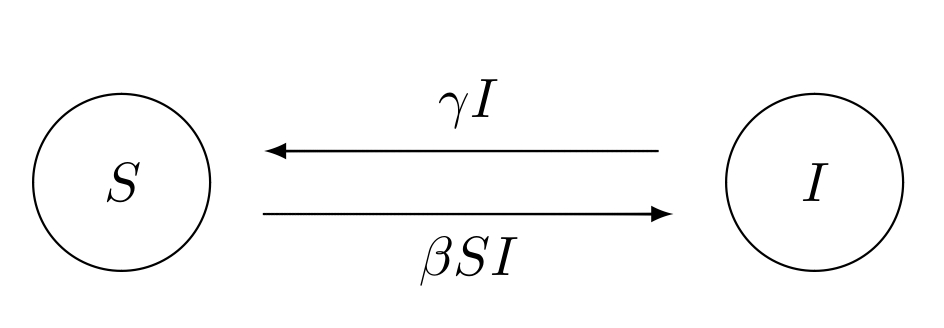
\includegraphics[width=\textwidth]{Figure1.jpg}
\caption{Dynamics of the SIS Model. Each susceptible individual is infected with rate $\beta I$, and each infective individual recovers with rate $\gamma$.}
\label{fig:1}
\end{figure}

\par We define the stochastic Markovian process ${\cal X}=\{S(t):\ t\geq0\}$, with
\begin{eqnarray*}
 S(t) &=& \hbox{\it ``number of susceptible individuals at time $t$''},\\
 I(t) &=& \hbox{\it ``number of infective individuals at time $t$''} \ = \ N-S(t),
\end{eqnarray*}
\par\noindent for $t\geq0$, which according to dynamics in Figure \ref{fig:1} is a birth-and-death process with absorbing state $S(t)=N$; see Figure \ref{fig:2}.
We consider an initially marked individual $A$ within the population, and our aim is to quantify the probability of individual $A$ suffering
at least one reinfection during the process. In order to compute this probability, we consider the extended process
${\cal X}^{ext}=\{{\bf X}^{ext}(t)=(S(t),A(t)):\ t\geq0\}$, where $A(t)$ represents the state of individual $A$ at time $t\geq0$, taking values
$S$, $S_I$ and $I$. These values represent that individual $A$, at time $t$, is susceptible and never suffered the disease before ($S$), is susceptible
but suffered the infection before ($S_I$) or is infective ($I$).

\par Moreover, we consider that individual $A$ might have an specific behaviour against the disease ({\it e.g.,} that individual $A$ recovers faster or
more slowly than the rest of the individuals, or that he/she has a different susceptibility and/or infectivity). Thus, we can define $\gamma(A)$ the recovery
rate of individual $A$, while individual $A$ infects any other individual in the population with rate $\beta_{A\rightarrow\bullet}$ and any other
individual infects $A$ with rate $\beta_{\bullet\rightarrow A}$. This introduces some heterogeneity in the population, allowing to compute the reinfection
probability of an individual when this individual is, for example, a super-spreader or a particularly susceptible individual within the population. We
note however that a completely homogeneous population can be studied just by setting $\gamma(A)=\gamma$ and $\beta_{\bullet\rightarrow A}=\beta_{A\rightarrow\bullet}=\beta$
in our analysis.
\begin{figure}
\centering
 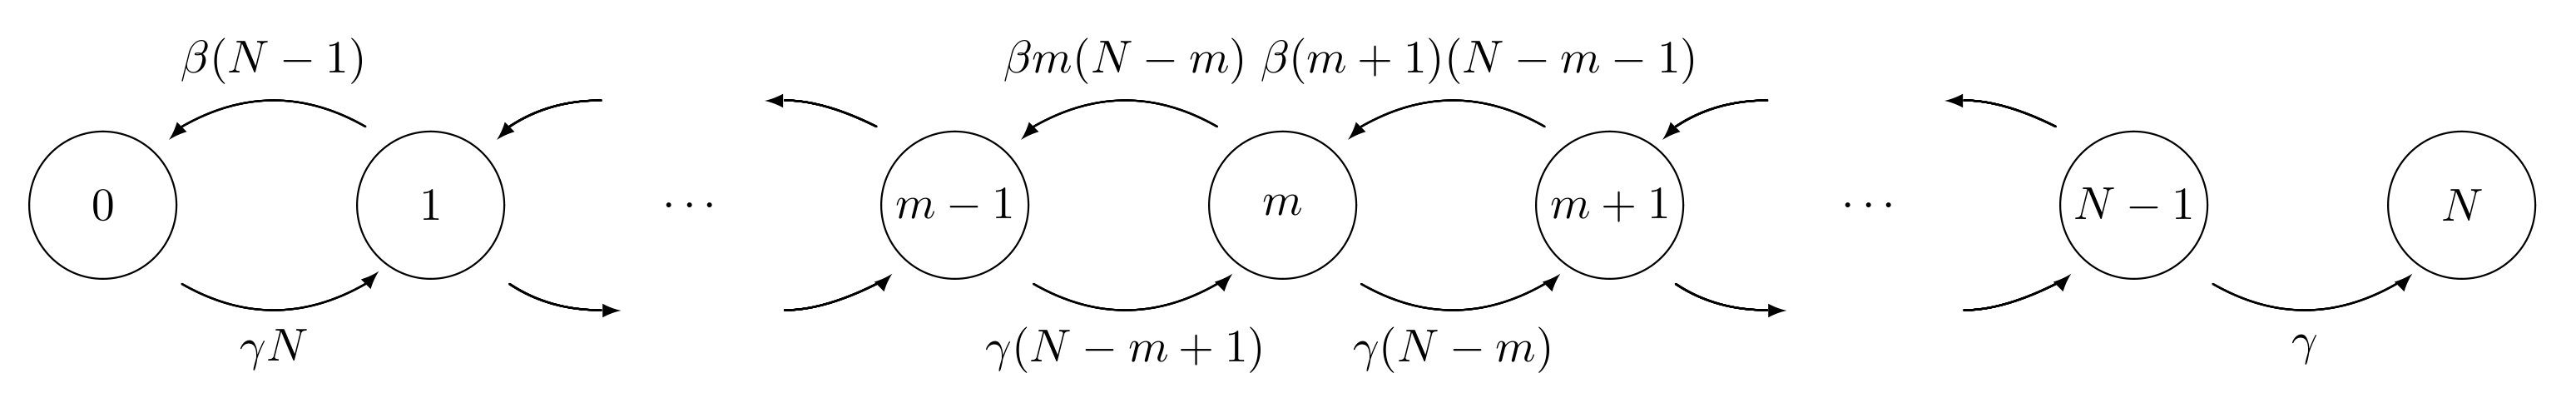
\includegraphics[width=\textwidth]{Figure2.jpg}
\caption{Birth-and-death process ${\cal X}$.}
\label{fig:2}
\end{figure}

\par We point out that extended process ${\cal X}^{ext}$ allows to: (i) consider an individual $A$ with individual associated rates $\beta_{A\rightarrow\bullet}$,
$\beta_{\bullet\rightarrow A}$ and $\gamma(A)$; (ii) keep track of the state of individual $A$ at any given time, which is necessary when computing the
reinfection probability of this individual. The state space of our extended process ${\cal X}^{ext}$ is given by
\begin{eqnarray*}
 {\cal S}^{ext} &=& \left(\{1,\dots,N-1\}\times\{S,S_I,I\}\right)\cup\{(0,I)\}\cup\left(\{N\}\times\{S,S_I\}\right)\cup\{\Delta\},
\end{eqnarray*}

\par\noindent where $\Delta$ is an {\it artificial} absorbing state representing the reinfection of individual $A$ for the first time, and $(N,S)$
and $(N,S_I)$ are absorbing states representing that the epidemic died out without individual $A$ suffering reinfection. Possible transitions between
states in ${\cal S}^{ext}$ are given in Table \ref{tab:1}, leading to the transitions diagram in Figure \ref{fig:3}.

\begin{table}
\centering
\begin{tabular}{|l|l|l|l|}
\hline
Type of event & Original state & Destination state & Rate\\
\hline
Recovery of an & $(m,S)$, $m\geq1$ & $(m+1,S)$ & $\gamma(N-m)$\\
infective individual & $(m,S_I)$, $m\geq1$ & $(m+1,S_I)$ & $\gamma(N-m)$\\
 & $(m,I)$ & $(m+1,S_I)$ & $\gamma(A)$\\
 & $(m,I)$, $m\leq N-2$ & $(m+1,I)$ & $\gamma(N-m-1)$\\
\hline
Infection of a & $(m,S)$, $m\geq1$ & $(m-1,I)$ & $\beta_{\bullet\rightarrow A}(N-m)$\\
susceptible individual & $(m,S)$, $m\geq1$ & $(m-1,S)$ & $\beta(m-1)(N-m)$\\
 & $(m,S_I)$, $m\geq1$ & $\Delta$ & $\beta_{\bullet\rightarrow A}(N-m)$\\
 & $(m,S_I)$, $m\geq1$ & $(m-1,S_I)$ & $\beta(m-1)(N-m)$\\
 & $(m,I)$ & $(m-1,I)$ & $\beta m(N-m-1)+\beta_{A\rightarrow\bullet}m$\\
\hline
\end{tabular}
\caption{Transitions and transition rates among states $(m,a)\in{\cal S}^{ext}$, for $0\leq m\leq N-1$, $n\geq1$.}
\label{tab:1}
\end{table}

\begin{figure}
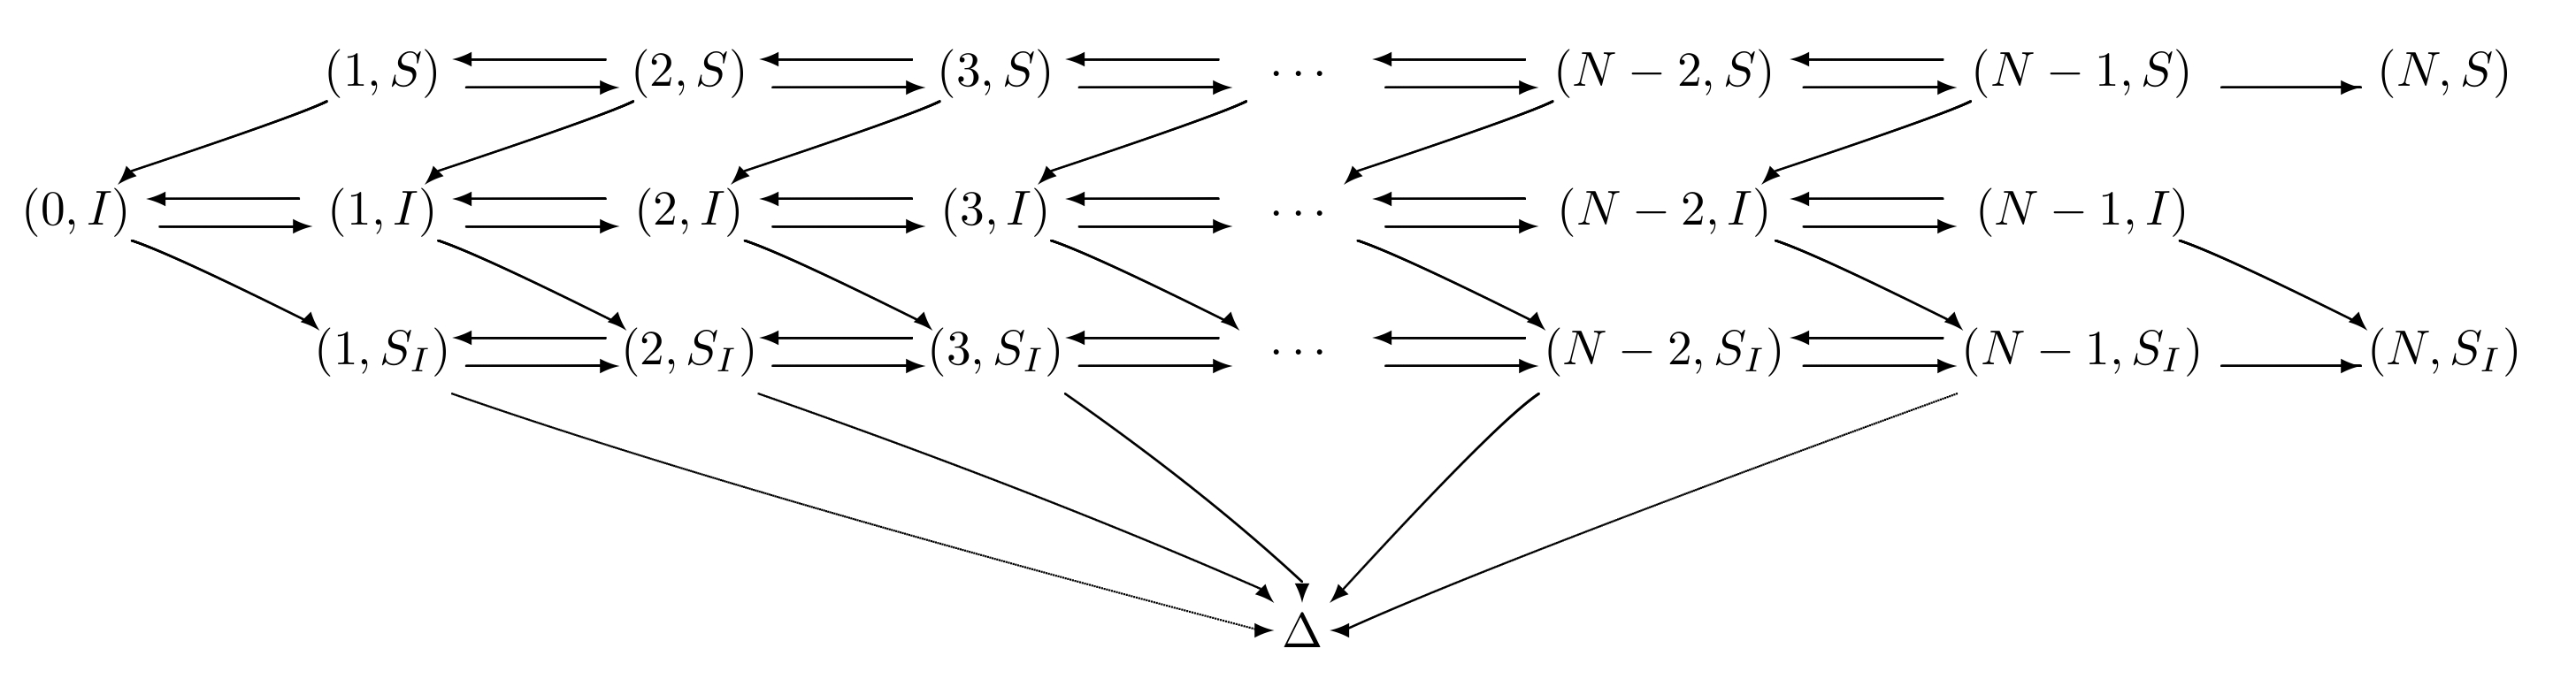
\includegraphics[width=\textwidth]{Figure3.jpg}
\caption{Transitions diagram for process ${\cal X}^{ext}$.}
\label{fig:3}
\end{figure}

\par Our interest is in computing
\begin{eqnarray*}
 p_{(m,a)} &=& \hbox{\it ``probability of individual $A$ suffering at least one reinfection}\\
&& \hbox{\it given the initial state of the process $(m,a)\in{\cal S}^{ext}$''},
\end{eqnarray*}
\par\noindent with trivial values $p_{\Delta}=1$, $p_{(N,S)}=p_{(N,S_I)}=0$. If the marked individual is the one starting the outbreak, we will focus on
the initial state $(m,a)=(N-1,I)$, while if the outbreak is initiated by a different individual the initial state to consider is $(m,a)=(N-1,S)$. Probabilities
$p_{(m,a)}$ for $(m,a)\in{\cal S}^{ext}$ satisfy the following equations, which can be obtained by implementing a first-step argument:
\begin{eqnarray}
 \theta_{(m,S)}p_{(m,S)} &=& \beta(m-1)(N-m)p_{(m-1,S)}+\beta_{\bullet\rightarrow A}(N-m)p_{(m-1,I)}\nonumber\\
&&+\gamma(N-m)p_{(m+1,S)},\quad 1\leq m\leq N-1,\label{eqn:1}\\
 \theta_{(m,I)}p_{(m,I)} &=& \left(\beta m(N-m-1)+\beta_{A\rightarrow\bullet}m\right)p_{(m-1,I)}+\gamma (N-m-1)p_{(m+1,I)}\nonumber\\
&&+\gamma(A)p_{(m+1,S_I)},\quad 0\leq m\leq N-1,\label{eqn:2}\\
 \theta_{(m,S)}p_{(m,S_I)} &=& \beta(m-1)(N-m)p_{(m-1,S_I)}+\beta_{\bullet\rightarrow A}(N-m)p_{\Delta}\nonumber\\
&&+\gamma(N-m)p_{(m+1,S_I)},\quad 1\leq m\leq N-1,\label{eqn:3}
\end{eqnarray}
\par\noindent with $\theta_{(m,S)}=\beta(m-1)(N-m)+\beta_{\bullet\rightarrow A}(N-m)+\gamma(N-m)$ and $\theta_{(m,I)}=\beta m(N-m-1)+\beta_{A\rightarrow\bullet}m+\gamma(N-m-1)+\gamma(A)$.
A preliminary analysis of Eqs. \eqref{eqn:1}-\eqref{eqn:3} allows us to find a recursive scheme for computing these probabilities. In particular,
Eq. \eqref{eqn:3} allows us to compute probabilities of the form $p_{(m,S_I)}$ which, once in hand, allow one for the computation of probabilities of
the form $p_{(m,I)}$ by Eq. \eqref{eqn:2}. Finally, once probabilities $p_{(m,I)}$ are in hand, Eq. \eqref{eqn:1} can be used to compute
probabilities of the form $p_{(m,S)}$; see {\bf Algorithm 1}.\\

%\par When solving Eq. \eqref{eqn:3}, it is possible (by using boundary conditions $p_{\Delta}=1$, $p_{(N,S_I)}=0$) to obtain the iterative
%scheme
%\begin{eqnarray*}
% p_{(N-1,S_I)} &=& h_{(N-1,S_I)}^{-1}\left(f_{(N-1,S_I)}p_{(N-2,S_I)}+g_{(N-1,S_I)}\right),\\
%&& \hbox{\it with } h_{(N-1,S_I)}=1,\ f_{(N-1,S_I)} ~=~ \frac{\beta(N-2)}{\theta_{(N-1,S_I)}},\ g_{(N-1,S_I)}=\frac{\beta_{\bullet\rightarrow A}}{\theta_{(N-1,S_I)}},\\
% p_{(m,S_I)} &=& h_{(m,S_I)}^{-1}\left(f_{(m,S_I)}p_{(m-1,S_I)}+g_{(m,S_I)}\right),\\
%&& \hbox{\it with } h_{(m,S_I)}=1-\frac{\gamma(N-m)}{\theta_{(m,S_I)}}h_{(m+1,S_I)}^{-1}f_{(m+1,S_I)},\ f_{(m,S_I)} ~=~ \frac{\beta(m-1)(N-m)}{\theta_{(m,S_I)}},\\
%&& g_{(m,S_I)}=\frac{\beta_{\bullet\rightarrow A}(N-m)}{\theta_{{(m,S_I)}}}+\frac{\gamma(N-m)}{\theta_{{(m,S_I)}}}h_{(m+1,S_I)}^{-1}g_{(m+1,S_I)}, \quad \hbox{\it for } m=N-2,\dots,2,\\
% p_{(1,S_I)} &=& h_{(1,S_I)}^{-1}g_{(1,S_I)},\\
%&& \hbox{\it with } h_{(1,S_I)}=1-\frac{\gamma(N-1)}{\theta_{(1,S_I)}}h_{(2,S_I)}^{-1}f_{(2,S_I)},\ g_{(1,S_I)}=\frac{\beta_{\bullet\rightarrow A} (N-1)}{\theta_{(1,S_I)}}+\frac{\gamma(N-1)}{\theta_{(1,S_I)}}h_{(2,S_I)}^{-1}g_{(2,S_I)},
%\end{eqnarray*}

%\par\noindent which yields an algorithmic procedure for computing these probabilities. Once these are in hand, Eq. \eqref{eqn:2} allows us to write
%\begin{eqnarray*}
% p_{(N-1,I)} &=& h_{(N-1,I)}^{-1}\left(f_{(N-1,I)}p_{(N-2,I)}+g_{(N-1,I)}\right),\\
%&& \hbox{\it with } h_{(N-1,I)}=1,\ f_{(N-1,I)}=\frac{\beta_{A\rightarrow\bullet}(N-1)}{\theta_{(N-1,I)}},\ g_{(N-1,I)}=\frac{\gamma(A)}{\theta_{(N-1,I)}}p_{(N,S_I)},\\
% p_{(m,I)} &=& h_{(m,I)}^{-1}\left(f_{(m,I)}p_{(m-1,I)}+g_{(m,I)}\right),\\
%&& \hbox{\it with } h_{(m,I)}=1-\frac{\gamma(N-m-1)}{\theta_{(m,I)}}h_{(m+1,I)}^{-1}f_{(m+1,I)},\ f_{(m,I)} ~=~ \frac{\beta m(N-m-1)+\beta_{A\rightarrow\bullet}m}{\theta_{(m,I)}},\\
%&& g_{(m,I)}=\frac{\gamma (N-m-1)}{\theta_{(m,I)}}h_{(m+1,I)}^{-1}g_{(m+1,I)}+\frac{\gamma(A)}{\theta_{(m,I)}}p_{(m+1,S_I)},\quad \hbox{\it for } m=N-2,\dots,1,\\
% p_{(0,I)} &=& h_{(0,I)}^{-1}g_{(0,I)},\\
%&& \hbox{\it with } h_{(0,I)}=1-\frac{\gamma(N-1)}{\theta_{(0,I)}}h_{(1,I)}^{-1}f_{(1,I)},\ g_{(0,I)}=\frac{\gamma(N-1)}{\theta_{(0,I)}}h_{(1,I)}^{-1}g_{(1,I)}+\frac{\gamma(A)}{\theta_{(0,I)}}p_{(1,S_I)}.
%\end{eqnarray*}

%\par\noindent Finally, probabilities of the form $p_{(m,S)}$ are obtained from Eq. \eqref{eqn:1} as
%\begin{eqnarray*}
% p_{(N-1,S)} &=& h_{(N-1,S)}^{-1}\left(f_{(N-1,S)}p_{(N-2,S)}+g_{(N-1,S)}\right),\ \hbox{\it with } h_{(N-1,S)}=1,\ f_{(N-1,S)} ~=~ \frac{\beta(N-2)}{\theta_{(N-1,S)}},\ g_{(N-1,S)}=\frac{\beta_{\bullet\rightarrow A}}{\theta_{(N-1,S)}}p_{(N-2,I)},\\
% p_{(m,S)} &=& h_{(m,S)}^{-1}\left(f_{(m,S)}p_{(m-1,S)}+g_{(m,S)}\right),\ \hbox{\it with } h_{(m,S)}=1-\frac{\gamma(N-m)}{\theta_{(m,S)}}h_{(m+1,S)}^{-1}f_{(m+1,S)},\ f_{(m,S)} ~=~ \frac{\beta (m-1)(N-m)}{\theta_{(m,S)}},\\
%&& g_{(m,S)}=\frac{\beta_{\bullet\rightarrow A}(N-m)}{\theta_{(m,S)}}p_{(m-1,I)}+\frac{\gamma(N-m)}{\theta_{(m,S)}}h_{(m+1,S)}^{-1}g_{(m+1,S)},\quad \hbox{\it for } m=N-2,\dots,2,\\
% p_{(1,S)} &=& h_{(1,S)}^{-1}g_{(1,S)},\ \hbox{\it with } h_{(1,S)}=1-\frac{\gamma(N-1)}{\theta_{(1,S)}}h_{(2,S)}^{-1}f_{(2,S)},\ g_{(1,S)}=\frac{\beta_{\bullet\rightarrow A} (N-1)}{\theta_{(1,S)}}p_{(0,I)}+\frac{\gamma(N-1)}{\theta_{(1,S)}}h_{(2,S)}^{-1}g_{(2,S)}.
%\end{eqnarray*}

%\par\noindent From previous recursions, {\bf Algorithm 1} is obtained for computing probabilities in Eqs. \eqref{eqn:1}-\eqref{eqn:3}.\\

\par\noindent{\bf Algorithm 1}
%\begin{minipage}{9cm}
\begin{description}
  \item \textit{\textbf{Recursive scheme for computing probabilities $p_{(m,S_I)}$ from Eq. \eqref{eqn:3}:}}
  \item $h_{(N-1,S)} ~=~ 1$;
  \item $f_{(N-1,S)} ~=~ \frac{\beta(N-2)}{\theta_{(N-1,S)}}$;
  \item $g_{(N-1,S_I)} ~=~ \frac{\beta_{\bullet\rightarrow A}}{\theta_{(N-1,S)}}$;
  \item \it For $m=N-2,\dots,1$:
  \item $~$\hspace{0.5cm} $h_{(m,S)} ~=~ 1-\frac{\gamma(N-m)}{\theta_{(m,S)}}h_{(m+1,S)}^{-1}f_{(m+1,S)}$;
  \item $~$\hspace{0.5cm} $f_{(m,S)} ~=~ \frac{\beta(m-1)(N-m)}{\theta_{(m,S)}}$;
  \item $~$\hspace{0.5cm} $g_{(m,S_I)} ~=~ \frac{\beta_{\bullet\rightarrow A}(N-m)}{\theta_{{(m,S)}}}+\frac{\gamma(N-m)}{\theta_{{(m,S)}}}h_{(m+1,S)}^{-1}g_{(m+1,S_I)}$;
  \item $p_{(1,S_I)} ~=~ h_{(1,S)}^{-1}g_{(1,S_I)}$;
  \item \it For $m=2,\dots,N-1$:
  \item $~$\hspace{0.5cm} $p_{(m,S_I)} ~=~ h_{(m,S)}^{-1}\left(f_{(m,S)}p_{(m-1,S_I)}+g_{(m,S_I)}\right)$;
  \item \textit{\textbf{Recursive scheme for computing probabilities $p_{(m,I)}$ from Eq. \eqref{eqn:2}:}}
  \item $h_{(N-1,I)} ~=~ 1$;
  \item $f_{(N-1,I)} ~=~ \frac{\beta_{A\rightarrow\bullet}(N-1)}{\theta_{(N-1,I)}}$;
  \item $g_{(N-1,I)} ~=~ \frac{\gamma(A)}{\theta_{(N-1,I)}}p_{(N,S_I)}$;
  \item \it For $m=N-2,\dots,0$:
  \item $~$\hspace{0.5cm} $h_{(m,I)} ~=~ 1-\frac{\gamma(N-m-1)}{\theta_{(m,I)}}h_{(m+1,I)}^{-1}f_{(m+1,I)}$;
  \item $~$\hspace{0.5cm} $f_{(m,I)} ~=~ \frac{\beta m(N-m-1)+\beta_{A\rightarrow\bullet}m}{\theta_{(m,I)}}$;
  \item $~$\hspace{0.5cm} $g_{(m,I)} ~=~ \frac{\gamma (N-m-1)}{\theta_{(m,I)}}h_{(m+1,I)}^{-1}g_{(m+1,I)}+\frac{\gamma(A)}{\theta_{(m,I)}}p_{(m+1,S_I)}$;
  \item $p_{(0,I)} ~=~ h_{(0,I)}^{-1}g_{(0,I)}$;
  \item \it For $m=1,\dots,N-1$:
  \item $~$\hspace{0.5cm} $p_{(m,I)} ~=~ h_{(m,I)}^{-1}\left(f_{(m,I)}p_{(m-1,I)}+g_{(m,I)}\right)$;
  \item \textit{\textbf{Recursive scheme for computing probabilities $p_{(m,S)}$ from Eq. \eqref{eqn:1}:}}
  \item $g_{(N-1,S)} ~=~ \frac{\beta_{\bullet\rightarrow A}}{\theta_{(N-1,S)}}p_{(N-2,I)}$;
  \item \it For $m=N-2,\dots,1$:
  \item $~$\hspace{0.5cm} $g_{(m,S)} ~=~ \frac{\beta_{\bullet\rightarrow A}(N-m)}{\theta_{(m,S)}}p_{(m-1,I)}+\frac{\gamma(N-m)}{\theta_{(m,S)}}h_{(m+1,S)}^{-1}g_{(m+1,S)}$;
  \item $p_{(1,S)} ~=~ h_{(1,S)}^{-1}g_{(1,S)}$;
  \item \it For $m=2,\dots,N-1$:
  \item $~$\hspace{0.5cm} $p_{(m,S)} ~=~ h_{(m,S)}^{-1}\left(f_{(m,S)}p_{(m-1,S)}+g_{(m,S)}\right)$;
\end{description}
%\end{minipage}

\subsection{Temporary and/or partial immunity SIR models}
\label{SubSect22}

\par We focus now on epidemic models where some kind of immunity is obtained by individuals after suffering the infection. To this aim, we consider models inspired from models in
Ref. \cite{gomes2004infection} where some temporary and/or partial immunity hypotheses are assumed:
\begin{itemize}
 \item {\it Temporary immunity:} upon infection, individuals develop an immune response leading to temporary immunity, which is lost after a certain
time.
  \item {\it Partial immunity:} individuals are protected while infected, and regain some susceptibility upon recovery.
\end{itemize}

\par\noindent As explained in \cite[Figure 1(e)]{gomes2004infection}, these hypotheses can be incorporated by considering a general model such as the one in Figure
\ref{fig:4}. Considering only partial immunity, or only temporary immunity, can be done by setting some of the model parameters in Figure \ref{fig:4} equal to zero. We refer for now to the model in Figure \ref{fig:4} as the {\it temporary-partial immunity SIR model} (TPI-SIR), and we will consider different immunity hypotheses in Section \ref{Sect3} by setting some model parameters equal to zero.
\begin{figure}
\centering
 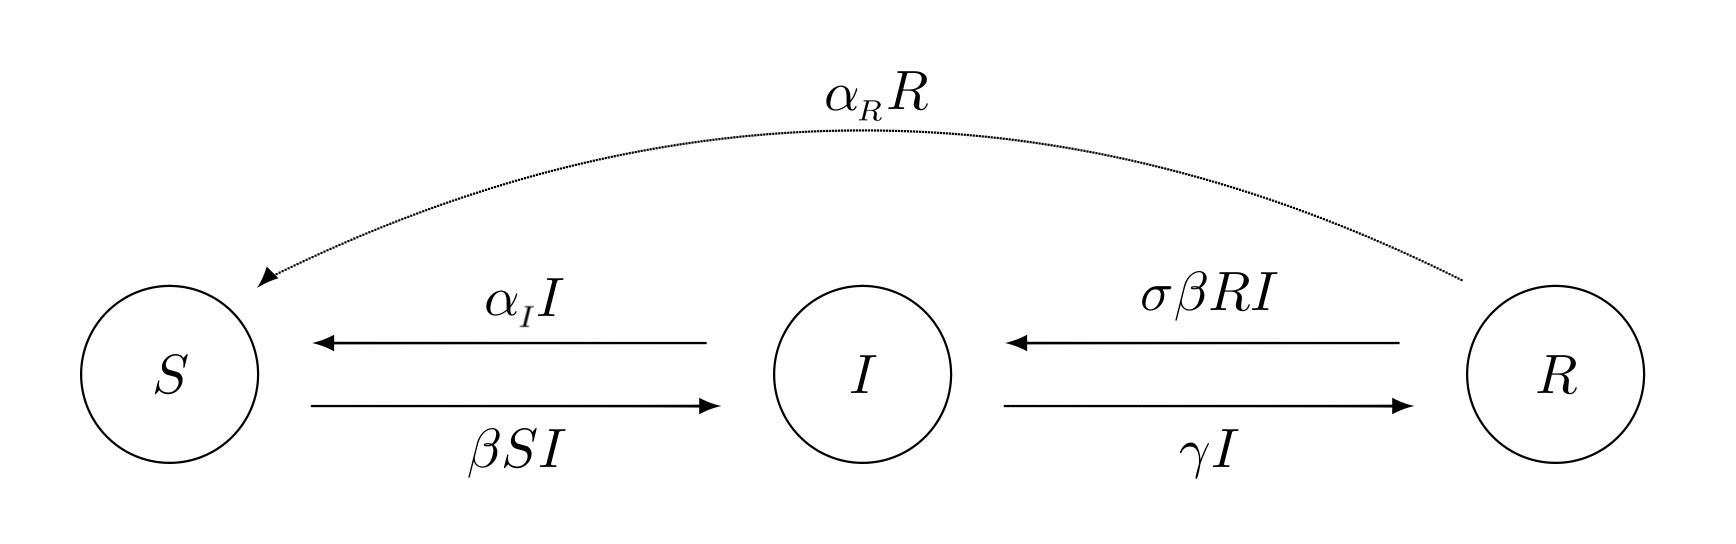
\includegraphics[width=\textwidth]{Figure4.jpg}
\caption{The {\it temporary-partial immunity SIR model} (TPI-SIR).}
\label{fig:4}
\end{figure}

\par We analyse in this section the probability of reinfection of a marked individual under the TPI-SIR Model. The TPI-SIR Model is represented by the Markovian
process ${\cal \tilde X}=\{{\bf \tilde X}(t)=({\tilde S}(t),{\tilde I}(t)):\ t\geq0\}$, with ${\tilde R}(t)=N-{\tilde S}(t)-{\tilde I}(t)$ the total
number of recovered individuals at time $t$, defined over the state space ${\cal \tilde S}=\{(m,n)\in\mathbb{N}^2_0: \ m+n\leq N\}$.
States of the form $(m,0)$ are considered as absorbing states representing the extinction of the epidemic; that is, we study the process only until
the epidemic dies out ({\it i.e.,} until ${\tilde I}(t)=0$), even thought according to Figure \ref{fig:4} there might still occur some events after that, only involving susceptible and recovered individuals.

\par We propose to track a marked individual $A$ by adding a third variable ${\tilde A}(t)$ to process ${\cal \tilde X}$ as in Subsection 2.1. In
particular, we consider the extended process ${\cal \tilde X}^{ext}=\{{\bf \tilde X}^{ext}(t)=({\tilde S}(t),{\tilde I}(t),{\tilde A}(t)):\ t\geq0\}$ where
${\tilde A}(t)$ takes values among states $\{S,S_I,I,R\}$ and represents the state of individual $A$ at time $t$ (that is, individual at time $t$ can be
susceptible having or not suffered the infection before, infected or recovered). The state space of
${\cal \tilde X}^{ext}$ is
\begin{eqnarray*}
 {\cal \tilde S}^{ext} &=& \left({\cal \tilde S}^{ext}(S)\times\{S,S_I\}\right)\cup\left({\cal \tilde S}^{ext}(I)\times\{I\}\right)\cup\left({\cal \tilde S}^{ext}(R)\times\{R\}\right)\cup\{\tilde \Delta\},
\end{eqnarray*}
\par\noindent ${\tilde \Delta}$ is an absorbing state representing reinfection of individual $A$ for the first time, and
\begin{eqnarray*}
{\cal \tilde S}^{ext}(S) &=& \{(m,n)\in\mathbb{N}_0^2:\ m>0,\ m+n\leq N\},\\
{\cal \tilde S}^{ext}(I) &=& \{(m,n)\in\mathbb{N}_0^2:\ n>0,\ m+n\leq N\},\\
{\cal \tilde S}^{ext}(R) &=& \{(m,n)\in\mathbb{N}_0^2:\ m+n<N\},
\end{eqnarray*}
\par\noindent relate to the possible numbers of susceptible and infective individuals in the population when individual A is susceptible, infective
or recovered, respectively. Transitions among states within ${\cal \tilde S}^{ext}$ are given in Table \ref{tab:2}, and individual $A$ is again considered to potentially
behave differently against the disease than the rest of individuals in the population, by considering individual rates $\beta_{\bullet\rightarrow A}$,
$\beta_{A\rightarrow\bullet}$, $\sigma(A)$, $\alpha_R(A)$, $\alpha_I(A)$ and $\gamma(A)$. In order to implement our methodology for a completely homogeneous
population, one would set $\beta_{\bullet\rightarrow A}=\beta_{A\rightarrow\bullet}=\beta$, $\gamma(A)=\gamma$, $\sigma(A)=\sigma$, $\alpha_R(A)=\alpha_R$ and $\alpha_I(A)=\alpha_I$.\\

\begin{table}
{\small
\centering
\begin{tabular}{|l|l|l|l|}
\hline
Event & Original state  & Destination state & Rate\\
 & & & \\
\hline
Recovery of & $(m,n,S)$, $m\geq1$ & $(m,n-1,S)$ & $\gamma n$\\
an infective & $(m,n,S_I)$, $m\geq1$ & $(m,n-1,S_I)$ & $\gamma n$\\
individual & $(m,n,I)$, $n\geq2$ & $(m,n-1,I)$ & $\gamma(n-1)$\\
 & $(m,n,I)$ & $(m,n-1,R)$ & $\gamma(A)$\\
 & $(m,n,R)$, $m+n<N$ & $(m,n-1,R)$ & $\gamma n$\\
\hline
Infection of & $(m,n,S)$, $m\geq1$ & $(m-1,n+1,I)$ & $\beta_{\bullet\rightarrow A}n$\\
a susceptible & $(m,n,S)$, $m\geq2$ & $(m-1,n+1,S)$ & $\beta(m-1)n$\\
individual & $(m,n,S_I)$, $m\geq1$ & ${\tilde \Delta}$ & $\beta_{\bullet\rightarrow A}n$\\
 & $(m,n,S_I)$, $m\geq2$ & $(m-1,n+1,S_I)$ & $\beta(m-1)n$\\
 & $(m,n,I)$, $m\geq1$ & $(m-1,n+1,I)$ & $\beta_{A\rightarrow\bullet}m+\beta(n-1)m$\\
 & $(m,n,R)$, $m\geq1,\ m+n<N$ & $(m-1,n+1,R)$ & $\beta mn$\\
\hline
Infection of & $(m,n,S)$, $m\geq1,\ m+n<N$ & $(m,n+1,S)$ & $\sigma\beta n(N-m-n)$\\
a recovered & $(m,n,S_I)$, $m\geq1$, $m+n<N$ & $(m,n+1,S_I)$ & $\sigma\beta n(N-m-n)$\\
individual & $(m,n,I)$, $m+n<N$ & $(m,n+1,I)$ & $\sigma\beta(n-1)(N-m-n)$\\
 & & & $+\sigma\beta_{A\rightarrow\bullet}(N-m-n)$\\
 & $(m,n,R)$, $m+n<N-1$ & $(m,n+1,R)$ & $\sigma\beta n(N-m-n-1)$\\
 & $(m,n,R)$, $m+n<N$ & ${\tilde \Delta}$ & $\sigma(A)\beta_{\bullet\rightarrow A} n$\\
\hline
Immunity loss & $(m,n,S)$, $m\geq1$ & $(m+1,n-1,S)$ & $\alpha_I n$\\
of an infective & $(m,n,S_I)$, $m\geq1$ & $(m+1,n-1,S_I)$ & $\alpha_I n$\\
individual & $(m,n,I)$, $n\geq2$ & $(m+1,n-1,I)$ & $\alpha_I(n-1)$\\
 & $(m,n,I)$ & $(m+1,n-1,S_I)$ & $\alpha_I(A)$\\
 & $(m,n,R)$, $m+n<N$ & $(m+1,n-1,R)$ & $\alpha_I n$\\
\hline
Immunity loss & $(m,n,S)$, $m\geq1,\ m+n<N$ & $(m+1,n,S)$ & $\alpha_R (N-m-n)$\\
of a recovered & $(m,n,S_I)$, $m\geq1,\ m+n<N$ & $(m+1,n,S_I)$ & $\alpha_R (N-m-n)$\\
individual & $(m,n,I)$, $m+n<N$ & $(m+1,n,I)$ & $\alpha_R (N-m-n)$\\
 & $(m,n,R)$, $m+n<N-1$ & $(m+1,n,R)$ & $\alpha_R (N-m-n-1)$\\
 & $(m,n,R)$, $m+n<N$ & $(m+1,n,S_I)$ & $\alpha_R(A)$\\
\hline
\end{tabular}
\caption{Transitions among states in ${\cal \tilde S}^{ext}$, for $n\geq1$, $m\geq0$, $m+n\leq N$.}
\label{tab:2}}
\end{table}

\par We define $p_{(m,n,a)}$ as the probability of individual $A$ suffering at least one reinfection given the initial state of the process
$(m,n,a)\in{\cal \tilde S}^{ext}$. These probabilities satisfy, for $m\geq0$, $n\geq1$ and $m+n\leq N$, equations
\begin{eqnarray}
 \theta_{(m,n,S)}p_{(m,n,S)} &=& \beta(m-1)np_{(m-1,n+1,S)}+\beta_{\bullet\rightarrow A}np_{(m-1,n+1,I)}+\gamma np_{(m,n-1,S)}\nonumber\\
&& +\alpha_I np_{(m+1,n-1,S)}+\alpha_R(N-m-n)p_{(m+1,n,S)}\nonumber\\
&&+\sigma\beta n(N-m-n)p_{(m,n+1,S)},\quad m\geq1,\label{eqn:4}\\
 \theta_{(m,n,I)}p_{(m,n,I)} &=& \left(\beta m(n-1)+\beta_{A\rightarrow\bullet}m\right)p_{(m-1,n+1,I)}+\gamma (n-1)p_{(m,n-1,I)}\nonumber\\
&& +\gamma(A)p_{(m,n-1,R)}+\alpha_I(n-1)p_{(m+1,n-1,I)}+\alpha_I(A)p_{(m+1,n-1,S_I)}\nonumber\\
&&+\left(\sigma\beta(n-1)(N-m-n)+\sigma\beta_{A\rightarrow\bullet}(N-m-n)\right)p_{(m,n+1,I)}\nonumber\\
&&+\alpha_R(N-m-n)p_{(m+1,n,I)},\quad \label{eqn:5}\\
 \theta_{(m,n,R)}p_{(m,n,R)} &=& \beta mnp_{(m-1,n+1,R)}+\gamma np_{(m,n-1,R)}+\alpha_I np_{(m+1,n-1,R)}\nonumber\\
&&+\alpha_R(N-m-n-1)p_{(m+1,n,R)}+\alpha_R(A)p_{(m+1,n,S_I)}+\sigma\beta n\nonumber\\
&&\times(N-m-n-1)p_{(m,n+1,R)}+\sigma(A)\beta_{\bullet\rightarrow A} np_{{\tilde \Delta}},\quad m+n< N,\label{eqn:6}\\
 \theta_{(m,n,S)}p_{(m,n,S_I)} &=& \beta(m-1)np_{(m-1,n+1,S_I)}+\beta_{\bullet\rightarrow A}np_{{\tilde \Delta}}+\gamma np_{(m,n-1,S_I)}\nonumber\\
&&+\alpha_I np_{(m+1,n-1,S_I)}+\alpha_R(N-m-n)p_{(m+1,n,S_I)}\nonumber\\
&&+\sigma\beta n(N-m-n)p_{(m,n+1,S_I)},\quad m\geq1,\label{eqn:7}
\end{eqnarray}
\par\noindent with $\theta_{(m,n,S)}=\beta(m-1)n+\beta_{\bullet\rightarrow A}n+\gamma n+\alpha_I n+\alpha_R(N-m-n)+\sigma\beta n(N-m-n)$, $\theta_{(m,n,I)}=\beta m(n-1)+\beta_{A\rightarrow\bullet}m+\gamma (n-1)+\gamma(A)+\alpha_I(n-1)+\alpha_I(A)+\sigma\beta(n-1)(N-m-n)+\sigma\beta_{A\rightarrow\bullet}(N-m-n)+\alpha_R(N-m-n)$, $\theta_{(m,n,R)}=\beta mn+\gamma n+\alpha_I n+\alpha_R(N-m-n-1)+\alpha_R(A)+\sigma\beta n(N-m-n-1)+\sigma(A)\beta_{\bullet\rightarrow A}n$, and boundary conditions $p_{{\tilde \Delta}}=1$, $p_{(m,0,S)}=p_{(m,0,S_I)}=p_{(m,0,R)}=0$, for any value of $m$.

\par Eqs. \eqref{eqn:4}-\eqref{eqn:7} can be solved algorithmically in a backwards fashion. In particular, Eq. \eqref{eqn:7} can be solved first by
considering
\begin{eqnarray*}
 {\cal \tilde S}^{ext}(S) &=& \{(m,n)\in\mathbb{N}_0^2:\ m>0,\ m+n\leq N\} \ = \ \left(\{(m,0):\ 1\leq m\leq N\}\right)\cup{\cal C}^{ext}(S),\\
 {\cal C}^{ext}(S) &=& \{(m,n)\in\mathbb{N}^2:\ m+n\leq N\} \ = \ \bigcup\limits_{k=2}^{N} L(S;k),\\
 L(S;k) &=& \{(m,n)\in\mathbb{N}^2:\ m+n=k\},\quad 2\leq k\leq N.
\end{eqnarray*}

\par\noindent With this states organisation, Eq. \eqref{eqn:7} can be written in matrix form as
\begin{eqnarray}\label{eqn:8}
 {\bf p}(S_I) &=& {\bf A}(S){\bf p}(S_I)+{\bf b}(S_I),
\end{eqnarray}
\par\noindent with
\begin{eqnarray*}
 {\bf p}(S_I) &=& \left(\begin{array}{c}
                         {\bf p}_2(S_I)\\
{\bf p}_3(S_I)\\
\vdots\\
{\bf p}_N(S_I)
\end{array}\right),\quad {\bf p}_k(S_I) \ = \ \left(\begin{array}{c}
p_{(k-1,1,S_I)}\\
p_{(k-2,2,S_I)}\\
\vdots\\
p_{(1,k-1,S_I)}
\end{array}\right),\\
{\bf b}(S_I) &=& \left(\begin{array}{c}
                          {\bf b}_2(S_I)\\
{\bf b}_3(S_I)\\
\vdots\\
{\bf b}_N(S_I)
                         \end{array}\right),\quad
{\bf b}_k(S_I) \ = \ \left(\begin{array}{c}
               \frac{\beta_{\bullet\rightarrow A}}{\theta_{(k-1,1,S)}}\\
\frac{\beta_{\bullet\rightarrow A}2}{\theta_{(k-2,2,S)}}\\
\vdots\\
\frac{\beta_{\bullet\rightarrow A}(k-1)}{\theta_{(1,k-1,S)}}\\
                         \end{array}\right),
\end{eqnarray*}

\par\noindent and with matrix ${\bf A}(S)$ given by
\begin{equation*}
  \left(\begin{array}{cccccc}
{\bf A}_{2,2}(S) & {\bf A}_{2,3}(S) & {\bf 0}_{J(S;2)\times J(S;4)} & \dots & {\bf 0}_{J(S;2)\times J(S;N-1)} & {\bf 0}_{J(S;2)\times J(S;N)}\\
{\bf A}_{3,2}(S) & {\bf A}_{3,3}(S) & {\bf A}_{3,4}(S) & \dots & {\bf 0}_{J(S;3)\times J(S;N-1)} & {\bf 0}_{J(S;3)\times J(S;N)}\\
{\bf 0}_{J(S;4)\times J(S;2)} & {\bf A}_{4,3}(S) & {\bf A}_{4,4}(S) & \dots & {\bf 0}_{J(S;4)\times J(S;N-1)} & {\bf 0}_{J(S;4)\times J(S;N)}\\
\vdots & \vdots & \vdots & \ddots & \vdots & \vdots\\
{\bf 0}_{J(S;N-1)\times J(S;2)} & {\bf 0}_{J(S;N-1)\times J(S;3)} & {\bf 0}_{J(S;N-1)\times J(S;4)} & \dots & {\bf A}_{N-1,N-1}(S) & {\bf A}_{N-1,N}(S) \\
{\bf 0}_{J(S;N)\times J(S;2)} & {\bf 0}_{J(S;N)\times J(S;3)} & {\bf 0}_{J(S;N)\times J(S;4)} & \dots & {\bf A}_{N,N-1}(S) & {\bf A}_{N,N}(S)
                        \end{array}\right),
\end{equation*}
\par\noindent and with sub-matrices
{\scriptsize
\begin{eqnarray*}
 {\bf A}_{k,k}(S) &=& \left(\begin{array}{cccccc}
0 & \frac{\beta(k-2)}{\theta_{(k-1,1,S)}} & 0 & \dots & 0 & 0\\
\frac{\alpha_I2}{\theta_{(k-2,2,S)}} & 0 & \frac{\beta2(k-3)}{\theta_{(k-2,2,S)}} & \dots & 0 & 0\\
0 & \frac{\alpha_I3}{\theta_{(k-3,3,S)}} & 0 & \dots & 0 & 0\\
\vdots & \vdots & \vdots & \ddots & \vdots & \vdots\\
0 & 0 & 0 & \dots & 0 & \frac{\beta(k-2)}{\theta_{(2,k-2,S)}}\\
0 & 0 & 0 & \dots & \frac{\alpha_I(k-1)}{\theta_{(1,k-1,S)}} & 0
                        \end{array}\right),\quad 2\leq k\leq N,\\
 {\bf A}_{k,k-1}(S) &=& \left(\begin{array}{cccccc}
0 & 0 & 0 & \dots & 0 & 0\\
\frac{\gamma2}{\theta_{(k-2,2,S)}} & 0 & 0 & \dots & 0 & 0\\
0 & \frac{\gamma3}{\theta_{(k-3,3,S)}} & 0 & \dots & 0 & 0\\
\vdots & \vdots & \vdots & \ddots & \vdots & \vdots\\
0 & 0 & 0 & \dots & \frac{\gamma(k-2)}{\theta_{(2,k-2,S)}} & 0\\
0 & 0 & 0 & \dots & 0 & \frac{\gamma(k-1)}{\theta_{(1,k-1,S)}}
                        \end{array}\right),\quad 3\leq k\leq N,
\end{eqnarray*}
\begin{eqnarray*}
 {\bf A}_{k,k+1}(S) &=& \left(\begin{array}{cccccc}
\frac{\alpha_R(N-k)}{\theta_{(k-1,1,S)}} & \frac{\sigma\beta(N-k)}{\theta_{(k-1,1,S)}} & 0 & \dots & 0 & 0\\
0 & \frac{\alpha_R(N-k)}{\theta_{(k-2,2,S)}} & \frac{\sigma\beta(N-k)2}{\theta_{(k-2,2,S)}} & \dots & 0 & 0\\
0 & 0 & \frac{\alpha_R(N-k)}{\theta_{(k-3,3,S)}} & \dots & 0 & 0\\
\vdots & \vdots & \vdots & \ddots & \vdots & \vdots\\
0 & 0 & 0 & \dots & \frac{\sigma\beta(N-k)(k-2)}{\theta_{(2,k-2,S)}} & 0\\
0 & 0 & 0 & \dots & \frac{\alpha_R(N-k)}{\theta_{(1,k-1,S)}} & \frac{\sigma\beta(N-k)(k-1)}{\theta_{(1,k-1,S)}}
                        \end{array}\right),\quad 2\leq k\leq N-1,
\end{eqnarray*}}

\par\noindent where $J(S;k)=\# L(S;k)=k-1$, and $\#B$ represents the cardinality of set $B$. According to the structure of matrix ${\bf A}(S)$,
system in Eq. \eqref{eqn:8} can be algorithmically solved in a specialised block-Gaussian elimination fashion; see {\bf Algorithm 2}.

\vspace{0.5cm}
\par \noindent{\bf Algorithm 2}
\begin{description}
  \item ${\bf H}_2(S) ~=~ {\bf I}_{J(S;2)}-{\bf A}_{2,2}(S)$;
  \item ${\bf J}_2(S_I) ~=~ {\bf b}_2(S_I)$;
  \item \it For $k=3,\dots,N$:
  \item $~$\hspace{0.5cm} ${\bf H}_k(S) ~=~ {\bf I}_{J(S;k)}-{\bf A}_{k,k}(S)-{\bf A}_{k,k-1}(S){\bf H}_{k-1}^{-1}(S){\bf A}_{k-1,k}(S)$;
  \item $~$\hspace{0.5cm} ${\bf J}_k(S_I) ~=~ {\bf A}_{k,k-1}(S){\bf H}_{k-1}^{-1}(S){\bf J}_{k-1}(S_I)+{\bf b}_k(S_I)$;
  \item ${\bf p}_N(S_I) ~=~ {\bf H}_N^{-1}(S){\bf J}_N(S_I)$;
  \item \it For $k=N-1,\dots,2$:
  \item $~$\hspace{0.5cm} ${\bf p}_k(S_I) ~=~ {\bf H}_k^{-1}(S)\left({\bf A}_{k,k+1}(S){\bf p}_{k+1}(S_I)+{\bf J}_k(S_I)\right)$;
\end{description}
\vspace{0.5cm}

\par Once probabilities of the form $p_{(m,n,S_I)}$ are in hand, one proceeds similarly to obtain probabilities $p_{(m,n,R)}$ from Eq. \eqref{eqn:6}, which can be
re-written in matrix form by organising
\begin{eqnarray*}
 {\cal \tilde S}^{ext}(R) &=& \{(m,n)\in\mathbb{N}_0^2:\ m+n< N\} \ = \ \left(\{(m,0):\ 0\leq m\leq N-1\}\right)\cup{\cal C}^{ext}(R),\\
 {\cal C}^{ext}(R) &=& \{(m,n)\in\mathbb{N}_0^2:\ n\geq1,\ m+n< N\} \ = \ \bigcup\limits_{k=1}^{N-1} L(R;k),\\
 L(R;k) &=& \{(m,n)\in\mathbb{N}_0^2:\ n\geq1,\ m+n=k\},\quad 1\leq k\leq N-1.
\end{eqnarray*}

\par\noindent In particular, we obtain
\begin{eqnarray}\label{eqn:9}
 {\bf p}(R) &=& {\bf A}(R){\bf p}(R)+{\bf b}(R),
\end{eqnarray}
\par\noindent with
\begin{eqnarray*}
 {\bf p}(R) &=& \left(\begin{array}{c}
                         {\bf p}_1(R)\\
{\bf p}_2(R)\\
\vdots\\
{\bf p}_{N-1}(R)
\end{array}\right),\quad {\bf p}_k(R) \ = \ \left(\begin{array}{c}
p_{(k-1,1,R)}\\
p_{(k-2,2,R)}\\
\vdots\\
p_{(1,k-1,R)}\\
p_{(0,k,R)}
\end{array}\right),
\end{eqnarray*}
\par\noindent column vector
\begin{eqnarray*}
{\bf b}(R) &=& \left(\begin{array}{c}
                          {\bf b}_1(R)\\
{\bf b}_2(R)\\
\vdots\\
{\bf b}_{N-1}(R)
                         \end{array}\right),\quad
{\bf b}_k(R) \ = \ \left(\begin{array}{c}
               \frac{\alpha_R(A)p_{(k,1,S_I)}+\sigma(A)\beta_{\bullet\rightarrow A}}{\theta_{(k-1,1,R)}}\\
\frac{\alpha_R(A)p_{(k-1,2,S_I)}+\sigma(A)\beta_{\bullet\rightarrow A}2}{\theta_{(k-2,2,R)}}\\
\vdots\\
\frac{\alpha_R(A)p_{(1,k,S_I)}+\sigma(A)\beta_{\bullet\rightarrow A}k}{\theta_{(0,k,R)}}
                         \end{array}\right),
\end{eqnarray*}

\par\noindent and with matrix ${\bf A}(R)$ given by
\begin{equation*}
  \left(\begin{array}{cccccc}
{\bf A}_{1,1}(R) & {\bf A}_{1,2}(R) & {\bf 0}_{J(R;1)\times J(R;3)} & \dots & {\bf 0}_{J(R;1)\times J(R;N-2)} & {\bf 0}_{J(R;1)\times J(R;N-1)}\\
{\bf A}_{2,1}(R) & {\bf A}_{2,2}(R) & {\bf A}_{2,3}(R) & \dots & {\bf 0}_{J(R;2)\times J(R;N-2)} & {\bf 0}_{J(R;2)\times J(R;N-1)}\\
{\bf 0}_{J(R;3)\times J(R;1)} & {\bf A}_{3,2}(R) & {\bf A}_{3,3}(R) & \dots & {\bf 0}_{J(R;3)\times J(R;N-2)} & {\bf 0}_{J(R;3)\times J(R;N-1)}\\
\vdots & \vdots & \vdots & \ddots & \vdots & \vdots\\
{\bf 0}_{J(R;N-2)\times J(R;1)} & {\bf 0}_{J(R;N-2)\times J(R;2)} & {\bf 0}_{J(R;N-2)\times J(R;3)} & \dots & {\bf A}_{N-2,N-2}(R) & {\bf A}_{N-2,N-1}(R) \\
{\bf 0}_{J(R;N-1)\times J(R;1)} & {\bf 0}_{J(R;N-1)\times J(R;2)} & {\bf 0}_{J(R;N-1)\times J(R;3)} & \dots & {\bf A}_{N-1,N-2}(R) & {\bf A}_{N-1,N-1}(R)
                        \end{array}\right),
\end{equation*}
\par\noindent with $J(R;k)=\#L(R;k)=k$. Finally, we have sub-matrices
{\scriptsize
\begin{eqnarray*}
 {\bf A}_{k,k}(R) &=& \left(\begin{array}{cccccc}
0 & \frac{\beta(k-1)}{\theta_{(k-1,1,R)}} & 0 & \dots & 0 & 0\\
\frac{\alpha_I2}{\theta_{(k-2,2,R)}} & 0 & \frac{\beta2(k-2)}{\theta_{(k-2,2,R)}} & \dots & 0 & 0\\
0 & \frac{\alpha_I3}{\theta_{(k-3,3,R)}} & 0 & \dots & 0 & 0\\
\vdots & \vdots & \vdots & \ddots & \vdots & \vdots\\
0 & 0 & 0 & \dots & 0 & \frac{\beta(k-1)}{\theta_{(1,k-1,R)}}\\
0 & 0 & 0 & \dots & \frac{\alpha_Ik}{\theta_{(0,k,R)}} & 0
                        \end{array}\right),\quad 1\leq k\leq N-1,\\
 {\bf A}_{k,k-1}(R) &=& \left(\begin{array}{cccccc}
0 & 0 & 0 & \dots & 0 & 0\\
\frac{\gamma2}{\theta_{(k-2,2,R)}} & 0 & 0 & \dots & 0 & 0\\
0 & \frac{\gamma3}{\theta_{(k-3,3,R)}} & 0 & \dots & 0 & 0\\
\vdots & \vdots & \vdots & \ddots & \vdots & \vdots\\
0 & 0 & 0 & \dots & \frac{\gamma(k-1)}{\theta_{(1,k-1,R)}} & 0\\
0 & 0 & 0 & \dots & 0 & \frac{\gamma k}{\theta_{(0,k,R)}}
                        \end{array}\right),\quad 2\leq k\leq N-1,\\
{\bf A}_{k,k+1}(R) &=& \left(\begin{array}{cccccc}
\frac{\alpha_R(N-k-1)}{\theta_{(k-1,1,R)}} & \frac{\sigma\beta(N-k-1)}{\theta_{(k-1,1,R)}} & 0 & \dots & 0 & 0\\
0 & \frac{\alpha_R(N-k-1)}{\theta_{(k-2,2,R)}} & \frac{\sigma\beta(N-k-1)2}{\theta_{(k-2,2,R)}} & \dots & 0 & 0\\
0 & 0 & \frac{\alpha_R(N-k-1)}{\theta_{(k-3,3,R)}} & \dots & 0 & 0\\
\vdots & \vdots & \vdots & \ddots & \vdots & \vdots\\
0 & 0 & 0 & \dots & \frac{\sigma\beta(N-k-1)(k-1)}{\theta_{(1,k-1,R)}} & 0\\
0 & 0 & 0 & \dots & \frac{\alpha_R(N-k-1)}{\theta_{(0,k,R)}} & \frac{\sigma\beta(N-k-1)k}{\theta_{(0,k,R)}}
                        \end{array}\right),\quad 1\leq k\leq N-2.
\end{eqnarray*}}

\par\noindent For solving Eq. \eqref{eqn:9} and the structure of matrix ${\bf A}(R)$, we construct {\bf Algorithm 2 (continuation I)}.

\vspace{0.5cm}
\par \noindent{\bf Algorithm 2 (continuation I)}
\begin{description}
  \item ${\bf H}_1(R) ~=~ {\bf I}_{J(R;1)}-{\bf A}_{1,1}(R)$;
  \item ${\bf J}_1(R) ~=~ {\bf b}_1(R)$;
  \item \it For $k=2,\dots,N-1$:
  \item $~$\hspace{0.5cm} ${\bf H}_k(R) ~=~ {\bf I}_{J(R;k)}-{\bf A}_{k,k}(R)-{\bf A}_{k,k-1}(R){\bf H}_{k-1}^{-1}(R){\bf A}_{k-1,k}(R)$;
  \item $~$\hspace{0.5cm} ${\bf J}_k(R) ~=~ {\bf A}_{k,k-1}(R){\bf H}_{k-1}^{-1}(R){\bf J}_{k-1}(R)+{\bf b}_k(R)$;
  \item ${\bf p}_{N-1}(R) ~=~ {\bf H}_{N-1}^{-1}(R){\bf J}_{N-1}(R)$;
  \item \it For $k=N-2,\dots,1$:
  \item $~$\hspace{0.5cm} ${\bf p}_k(R) ~=~ {\bf H}_k^{-1}(R)\left({\bf A}_{k,k+1}(R){\bf p}_{k+1}(R)+{\bf J}_k(R)\right)$;
\end{description}
\vspace{0.5cm}

\par In a similar way, probabilities of the form $p_{(m,n,I)}$ can be obtained from Eq. \eqref{eqn:5} once both probabilities of the form
$p_{(m,n,S_I)}$ and $p_{(m,n,R)}$ are in hand. In particular, by organising
\begin{eqnarray*}
 {\cal \tilde S}^{ext}(I) &=& \{(m,n)\in\mathbb{N}_0^2:\ n\geq1,\ m+n\leq N\} \ = \ {\cal C}^{ext}(I),\\
 {\cal C}^{ext}(I) &=& \bigcup\limits_{k=1}^{N} L(I;k),\\
 L(I;k) &=& \{(m,n)\in\mathbb{N}_0^2:\ n\geq1,\ m+n=k\},\quad 1\leq k\leq N,
\end{eqnarray*}

\par\noindent we obtain
\begin{eqnarray}\label{eqn:10}
 {\bf p}(I) &=& {\bf A}(I){\bf p}(I)+{\bf b}(I),
\end{eqnarray}
\par\noindent with
\begin{eqnarray*}
 {\bf p}(I) &=& \left(\begin{array}{c}
                         {\bf p}_1(I)\\
{\bf p}_2(I)\\
\vdots\\
{\bf p}_{N}(I)
\end{array}\right),\quad {\bf p}_k(I) \ = \ \left(\begin{array}{c}
p_{(k-1,1,I)}\\
p_{(k-2,2,I)}\\
\vdots\\
p_{(1,k-1,I)}\\
p_{(0,k,I)}
\end{array}\right),
\end{eqnarray*}
\par\noindent column vector
\begin{eqnarray*}
{\bf b}(I) &=& \left(\begin{array}{c}
                          {\bf b}_1(I)\\
{\bf b}_2(I)\\
\vdots\\
{\bf b}_{N}(I)
                         \end{array}\right),\quad
{\bf b}_k(I) \ = \ \left(\begin{array}{c}
               0\\
\frac{\gamma(A) p_{(k-2,1,R)}+\alpha_I(A) p_{(k-1,1,S_I)}}{\theta_{(k-2,2,I)}}\\
\vdots\\
\frac{\gamma(A)p_{(0,k-1,R)}+\alpha_I(A)p_{(1,k-1,S_I)}}{\theta_{(0,k,I)}}
                         \end{array}\right),
\end{eqnarray*}

\par\noindent and with matrix ${\bf A}(I)$ given by
\begin{equation*}
  \left(\begin{array}{cccccc}
{\bf A}_{1,1}(I) & {\bf A}_{1,2}(I) & {\bf 0}_{J(I;1)\times J(I;3)} & \dots & {\bf 0}_{J(I;1)\times J(I;N-1)} & {\bf 0}_{J(I;1)\times J(I;N)}\\
{\bf A}_{2,1}(I) & {\bf A}_{2,2}(I) & {\bf A}_{2,3}(I) & \dots & {\bf 0}_{J(I;2)\times J(I;N-1)} & {\bf 0}_{J(I;2)\times J(I;N)}\\
{\bf 0}_{J(I;3)\times J(I;1)} & {\bf A}_{3,2}(I) & {\bf A}_{3,3}(I) & \dots & {\bf 0}_{J(I;3)\times J(I;N-1)} & {\bf 0}_{J(I;3)\times J(I;N)}\\
\vdots & \vdots & \vdots & \ddots & \vdots & \vdots\\
{\bf 0}_{J(I;N-1)\times J(I;1)} & {\bf 0}_{J(I;N-1)\times J(I;2)} & {\bf 0}_{J(I;N-1)\times J(I;3)} & \dots & {\bf A}_{N-1,N-1}(I) & {\bf A}_{N-1,N}(I) \\
{\bf 0}_{J(I;N)\times J(I;1)} & {\bf 0}_{J(I;N)\times J(I;2)} & {\bf 0}_{J(I;N)\times J(I;3)} & \dots & {\bf A}_{N,N-1}(I) & {\bf A}_{N,N}(I)
                        \end{array}\right),
\end{equation*}
\par\noindent with $J(I;k)=\#L(I;k)=k$. Finally, sub-matrices are given as
{\scriptsize
\begin{eqnarray*}
 {\bf A}_{k,k}(I) &=& \left(\begin{array}{cccccc}
0 & \frac{\beta_{A\rightarrow\bullet}(k-1)}{\theta_{(k-1,1,I)}} & 0 & \dots & 0 & 0\\
\frac{\alpha_I}{\theta_{(k-2,2,I)}} & 0 & \frac{(\beta_{A\rightarrow\bullet}+\beta)(k-2)}{\theta_{(k-2,2,I)}} & \dots & 0 & 0\\
0 & \frac{\alpha_I2}{\theta_{(k-3,3,I)}} & 0 & \dots & 0 & 0\\
\vdots & \vdots & \vdots & \ddots & \vdots & \vdots\\
0 & 0 & 0 & \dots & 0 & \frac{\beta_{A\rightarrow\bullet}+\beta(k-2)}{\theta_{(1,k-1,I)}}\\
0 & 0 & 0 & \dots & \frac{\alpha_I (k-1)}{\theta_{(0,k,I)}} & 0
                        \end{array}\right),\quad 1\leq k\leq N,\\
 {\bf A}_{k,k-1}(I) &=& \left(\begin{array}{cccccc}
0 & 0 & 0 & \dots & 0 & 0\\
\frac{\gamma}{\theta_{(k-2,2,I)}} & 0 & 0 & \dots & 0 & 0\\
0 & \frac{\gamma2}{\theta_{(k-3,3,I)}} & 0 & \dots & 0 & 0\\
\vdots & \vdots & \vdots & \ddots & \vdots & \vdots\\
0 & 0 & 0 & \dots & \frac{\gamma(k-2)}{\theta_{(1,k-1,I)}} & 0\\
0 & 0 & 0 & \dots & 0 & \frac{\gamma (k-1)}{\theta_{(0,k,I)}}
                        \end{array}\right),\quad 2\leq k\leq N,\\
 {\bf A}_{k,k+1}(I) &=& \left(\begin{array}{cccccc}
\frac{\alpha_R(N-k)}{\theta_{(k-1,1,I)}} & \frac{\sigma(N-k)\beta_{A\rightarrow\bullet}}{\theta_{(k-1,1,I)}} & 0 & \dots & 0 & 0\\
0 & \frac{\alpha_R(N-k)}{\theta_{(k-2,2,I)}} & \frac{\sigma(N-k)(\beta+\beta_{A\rightarrow\bullet})}{\theta_{(k-2,2,I)}} & \dots & 0 & 0\\
0 & 0 & \frac{\alpha_R(N-k)}{\theta_{(k-3,3,I)}} & \dots & 0 & 0\\
\vdots & \vdots & \vdots & \ddots & \vdots & \vdots\\
0 & 0 & 0 & \dots & \frac{\sigma(N-k)(\beta(k-2)+\beta_{A\rightarrow\bullet})}{\theta_{(1,k-1,I)}} & 0\\
0 & 0 & 0 & \dots & \frac{\alpha_R(N-k)}{\theta_{(0,k,I)}} & \frac{\sigma(N-k)(\beta(k-1)+\beta_{A\rightarrow\bullet})}{\theta_{(0,k,I)}}
                        \end{array}\right),\\
                        && \quad\quad\quad\quad\quad\quad\quad\quad\quad\quad\quad\quad\quad\quad\quad\quad\quad\quad\quad\quad\quad\quad\quad\quad\quad\quad\quad\quad\quad\quad\quad\quad\quad\quad\quad\quad\quad\quad\quad\quad\quad\quad\quad 1\leq k\leq N-1.
\end{eqnarray*}}

\par\noindent From Eq. \eqref{eqn:10}, we construct {\bf Algorithm 2 (continuation II)}.\\

\vspace{0.5cm}
\par \noindent{\bf Algorithm 2 (continuation II)}
\begin{description}
  \item ${\bf H}_1(I) ~=~ {\bf I}_{J(I;1)}-{\bf A}_{1,1}(I)$;
  \item ${\bf J}_1(I) ~=~ {\bf b}_1(I)$;
  \item \it For $k=2,\dots,N$:
  \item $~$\hspace{0.5cm} ${\bf H}_k(I) ~=~ {\bf I}_{J(I;k)}-{\bf A}_{k,k}(I)-{\bf A}_{k,k-1}(I){\bf H}_{k-1}^{-1}(I){\bf A}_{k-1,k}(I)$;
  \item $~$\hspace{0.5cm} ${\bf J}_k(I) ~=~ {\bf A}_{k,k-1}(I){\bf H}_{k-1}^{-1}(I){\bf J}_{k-1}(I)+{\bf b}_k(I)$;
  \item ${\bf p}_{N}(I) ~=~ {\bf H}_{N}^{-1}(I){\bf J}_{N}(I)$;
  \item \it For $k=N-1,\dots,1$:
  \item $~$\hspace{0.5cm} ${\bf p}_k(I) ~=~ {\bf H}_k^{-1}(I)\left({\bf A}_{k,k+1}(I){\bf p}_{k+1}(I)+{\bf J}_k(I)\right)$;
\end{description}
\vspace{0.5cm}

\par Finally, probabilities $p_{(m,n,S)}$ can be computed from Eq. \eqref{eqn:4} by following exactly the same arguments than the ones used for solving Eq. \eqref{eqn:7}. In
particular, we note that Eqs. \eqref{eqn:4} and \eqref{eqn:7} only differ in addends $\beta_{\bullet\rightarrow A}np_{{\tilde \Delta}}$ (in Eq. \eqref{eqn:7})
and $\beta_{\bullet\rightarrow A}np_{(m-1,n+1,I)}$ (in Eq. \eqref{eqn:4}). Thus, first steps of {\bf Algorithm 2} directly apply for solving
Eq. \eqref{eqn:4}, using same matrices ${\bf A}_{k,k'}(S)$, but with new vector ${\bf b}(S)$ instead of ${\bf b}(S_I)$,
\begin{eqnarray*}
{\bf b}(S) &=& \left(\begin{array}{c}
                          {\bf b}_2(S)\\
{\bf b}_3(S)\\
\vdots\\
{\bf b}_N(S)
                         \end{array}\right),\quad
{\bf b}_k(S) \ = \ \left(\begin{array}{c}
               \frac{\beta_{\bullet\rightarrow A}p_{(k-2,2,I)}}{\theta_{(k-1,1,S)}}\\
\frac{\beta_{\bullet\rightarrow A}2p_{(k-3,3,I)}}{\theta_{(k-2,2,S)}}\\
\vdots\\
\frac{\beta_{\bullet\rightarrow A}(k-1)p_{(0,k,I)}}{\theta_{(1,k-1,S)}}\\
                         \end{array}\right).
\end{eqnarray*}
%\subsection{Local Sensitivity Analysis}

%\par Once probabilities $p_{(m,a)}$, for $a\in\{S,S_I,I\}$ (ND-SIS Model), and $p_{(m,n,a)}$, for $a\in\{S,S_I,I,R\}$ (TPI-SIR, TI-SIR and PI-SIR Models),
%are in hand, a particular question that arises is the role played by each of the parameter values in these reinfection probabilities. In particular,
%given particular values of the parameters $\beta$, $\gamma$, $\alpha_I$, $\alpha_R$ and $\sigma$, our interest here is to analyse the impact that perturbations of
%these values have on the reinfection probabilities. A particular feature of our analysis in previous sections is that it allows to compute, in order
%to address this question, the exact partial derivatives of the reinfection probabilities with respect the parameters under study.

%\subsubsection{ND-SIS Model}

%\par We have computed in Section 2 the probabilities of the form $p_{(m,a)}$ with $a\in\{S,S_I,I\}$, by solving the system of equations given by
%Eqs. \eqref{eqn:1}-\eqref{eqn:3}. One may obtain the partial derivatives of interest $\frac{\partial p_{(m,a)}}{\partial w}$, for $w\in\{\beta,\gamma\}$, by
%means of differentiating this system. In particular, these partial derivatives verify:

%\begin{eqnarray}
%  \theta_{m}\frac{\partial p_{(m,S)}}{\partial w} &=& \beta m(N-m){\bar i_m}\frac{\partial p_{(m-1,S)}}{\partial w}+\beta m(N-m)i_m\frac{\partial p_{(m-1,I)}}{\partial w}+\gamma(N-m)\frac{\partial %p_{(m+1,S)}}{\partial w}+\frac{\partial(\beta m(N-m){\bar i_m})}{\partial w} p_{(m-1,S)}\nonumber\\
%&& +\frac{\partial(\beta m(N-m)i_m)}{\partial w} p_{(m-1,I)}+\frac{\partial (\gamma(N-m))}{\partial w}p_{(m+1,S)}-\frac{\partial \theta_m}{\partial w}p_{(m,S)},\quad 1\leq m\leq %N-1,\label{eqn:1s}\\
% \theta_{m}\frac{\partial p_{(m,I)}}{\partial w} &=& \beta m(N-m)\frac{\partial p_{(m-1,I)}}{\partial w}+\gamma (N-m){\bar s_m}\frac{\partial p_{(m+1,I)}}{\partial w}+\gamma(N-m)s_m\frac{\partial %p_{(m+1,S_I)}}{\partial w}+\frac{\partial(\beta m(N-m))}{\partial w}p_{(m-1,I)}\nonumber \\
%&& + \frac{\partial(\gamma (N-m){\bar s_m})}{\partial w}p_{(m+1,I)}+\frac{\partial (\gamma(N-m)s_m)}{\partial w}p_{(m+1,S_I)}-\frac{\partial \theta_m}{\partial w}p_{(m,I)},\quad 0\leq m\leq %N-1,\label{eqn:2s}\\
% \theta_{m}\frac{\partial p_{(m,S_I)}}{\partial w} &=& \beta m(N-m){\bar i_m}\frac{\partial p_{(m-1,S_I)}}{\partial w}+\gamma(N-m)\frac{\partial p_{(m+1,S_I)}}{\partial w}+\frac{\partial (\beta %m(N-m){\bar i_m})}{\partial w}p_{(m-1,S_I)}+\frac{\partial( \beta m(N-m)i_m)}{\partial w}\nonumber\\
%&& +\frac{\partial(\gamma (N-m))}{\partial w}p_{(m+1,S_I)}-\frac{\partial \theta_m}{\partial w}p_{(m,S_I)},\quad 1\leq m\leq N-1.\label{eqn:3s}
%\end{eqnarray}

%\par For solving \eqref{eqn:1s}-\eqref{eqn:3s}, one may adapt Algorithm 1. In particular, this can be straightforwardly done by directly differentiating
%steps in this algorithm, so that Algorithm 1S is obtained, which computes the partial derivatives $\frac{\partial p_{(m,a)}}{\partial w}$, for $w\in\{\beta,\gamma\}$,
%$a\in\{S,S_I,I\}$. In Algorithm 1S, $h_{k}^{(i,w)}$, $f_{k}^{(i,w)}$, and $g_{k}^{(i,w)}$ represent $\frac{\partial h_{k}^{(i)}}{\partial w}$, $\frac{\partial f_{k}^{(i)}}{\partial w}$
%and $\frac{\partial g_{k}^{(i)}}{\partial w}$, respectively (for $i\in\{1,2,3\}$).

%\vspace{0.5cm}
%\par \noindent{\bf Algorithm 1S}

%\begin{description}
%  \item $h_{N-1}^{(3,w)} ~=~ 0$;
%  \item $f_{N-1}^{(3,w)} ~=~ \left\{\begin{array}{ll}
%                                     \frac{(N-1){\bar i_{N-1}}\theta_{N-1}-\beta(N-1)^2{\bar i_{N-1}}}{\theta_{N-1}^2},& \hbox{\it if $w=\beta$,}\\
%-\frac{\beta(N-1){\bar i_{N-1}}}{\theta_{N-1}^2},& \hbox{\it if $w=\gamma$};
%                                    \end{array}\right.$
%  \item $g_{N-1}^{(3,w)} ~=~ \left\{\begin{array}{ll}
%                                     \frac{(N-1)i_{N-1}\theta_{N-1}-\beta(N-1)^2i_{N-1}}{\theta_{N-1}^2},& \hbox{\it if $w=\beta$,}\\
%-\frac{\beta(N-1)i_{N-1}}{\theta_{N-1}^2},& \hbox{\it if $w=\gamma$};
%                                    \end{array}\right.$
%  \item \it For $m=N-2,\dots,1$:
%  \item $~$\hspace{0.5cm} $h_{m}^{(3,w)} ~=~ \left\{\begin{array}{ll}
%\frac{\gamma(N-m)^2m}{\theta_m^2}\bullet\frac{f_{m+1}^{(3)}}{h_{m+1}^{(3)}}-\frac{\gamma(N-m)}{\theta_m}\bullet\frac{f_{m+1}^{(3,w)}h_{m+1}^{(3)}-f_{m+1}^{(3)}h_{m+1}^{(3,w)}}{(h_{m+1}^{(3)})^2},& %\hbox{\it if $w=\beta$},\\
%-\frac{(N-m)\theta_m-\gamma(N-m)^2}{\theta_m^2}\bullet\frac{f_{m+1}^{(3)}}{h_{m+1}^{(3)}}-\frac{\gamma(N-m)}{\theta_m}\bullet\frac{f_{m+1}^{(3,w)}h_{m+1}^{(3)}-f_{m+1}^{(3)}h_{m+1}^{(3,w)}}{(h_{m+1}^{(3)})^2},& %\hbox{\it if $w=\gamma$};
%                                                    \end{array}\right.$
%  \item $~$\hspace{0.5cm} $f_{m}^{(3,w)} ~=~ \left\{\begin{array}{ll}
%\frac{m(N-m){\bar i_m}\theta_m-\beta m^2(N-m)^2{\bar i_m}}{\theta_m^2},& \hbox{\it if $w=\beta$},\\
%-\frac{\beta m(N-m)^2{\bar i_m}}{\theta_m^2},& \hbox{\it if $w=\gamma$};
%                                                   \end{array}\right.$
%  \item $~$\hspace{0.5cm} $g_{m}^{(3,w)} ~=~ \left\{\begin{array}{ll}
%-\frac{\gamma(N-m)^2m}{\theta_m^2}\bullet %\frac{g_{m+1}^{(3)}}{h_{m+1}^{(3)}}+\frac{\gamma(N-m)}{\theta_m}\bullet\frac{g_{m+1}^{(3,w)}h_{m+1}^{(3)}-g_{m+1}^{(3)}h_{m+1}^{(3,w)}}{(h_{m+1}^{(3)})^2}+\frac{m(N-m)i_m\theta_m-\beta %m^2(N-m)^2i_m}{\theta_m^2},& \hbox{\it if $w=\beta$},\\
%\frac{(N-m)\theta_m-\gamma(N-m)^2}{\theta_m^2}\bullet \frac{g_{m+1}^{(3)}}{h_{m+1}^{(3)}}+\frac{\gamma(N-m)}{\theta_m}\bullet\frac{g_{m+1}^{(3,w)}h_{m+1}^{(3)}-g_{m+1}^{(3)}h_{m+1}^{(3,w)}}{(h_{m+1}^{(3)})^2}-\frac{\beta m(N-m)^2i_m}{\theta_m^2},& \hbox{\it if $w=\gamma$};
%                                                   \end{array}\right.$
%  \item $\frac{\partial p_{(1,S_I)}}{\partial w} ~=~ \frac{g_1^{(3,w)}h_1^{(3)}-g_1^{(3)}h_1^{(3,w)}}{(h_{1}^{(3)})^2}$;
%  \item \it For $m=2,\dots,N-1$:
%  \item $~$\hspace{0.5cm} $\frac{\partial p_{(m,S_I)}}{\partial w} ~=~ h_{m}^{(3)^{-1}}\left(f_{m}^{(3,w)}p_{(m-1,S_I)}+f_{m}^{(3)}\frac{\partial p_{(m-1,S_I)}}{\partial w}+g_{m}^{(3,w)}-h_m^{(3,w)}p_{(m,S_I)}\right)$;
%  \item (continuation I)
%  \item $h_{N-1}^{(2,w)} ~=~ 0$;
%  \item $f_{N-1}^{(2,w)} ~=~ \left\{\begin{array}{ll}
%                                     \frac{(N-1)\theta_{N-1}-\beta(N-1)^2}{\theta_{N-1}^2},& \hbox{\it if $w=\beta$,}\\
%-\frac{\beta(N-1)}{\theta_{N-1}^2},& \hbox{\it if $w=\gamma$};
%                                    \end{array}\right.$
%  \item $g_{N-1}^{(2,w)} ~=~ 0$;
%  \item \it For $m=N-2,\dots,0$:
%  \item $~$\hspace{0.5cm} $h_{m}^{(2,w)} ~=~ \left\{\begin{array}{ll}
%\frac{\gamma(N-m)^2m{\bar s_m}}{\theta_m^2}\bullet\frac{f_{m+1}^{(2)}}{h_{m+1}^{(2)}}-\frac{\gamma(N-m){\bar s_m}}{\theta_m}\bullet\frac{f_{m+1}^{(2,w)}h_{m+1}^{(2)}-f_{m+1}^{(2)}h_{m+1}^{(2,w)}}{(h_{m+1}^{(2)})^2},& \hbox{\it if $w=\beta$},\\
%-\frac{(N-m){\bar s_m}\theta_m-\gamma(N-m)^2{\bar s_m}}{\theta_m^2}\bullet\frac{f_{m+1}^{(2)}}{h_{m+1}^{(2)}}-\frac{\gamma(N-m){\bar s_m}}{\theta_m}\bullet\frac{f_{m+1}^{(2,w)}h_{m+1}^{(2)}-f_{m+1}^{(2)}h_{m+1}^{(2,w)}}{(h_{m+1}^{(2)})^2},& \hbox{\it if $w=\gamma$};
%                                                    \end{array}\right.$
%  \item $~$\hspace{0.5cm} $f_{m}^{(2,w)} ~=~ \left\{\begin{array}{ll}
%\frac{m(N-m)\theta_m-\beta m^2(N-m)^2}{\theta_m^2},& \hbox{\it if $w=\beta$},\\
%-\frac{\beta m(N-m)^2}{\theta_m^2},& \hbox{\it if $w=\gamma$};
%                                                   \end{array}\right.$
%  \item $~$\hspace{0.5cm} $g_{m}^{(2,w)} ~=~ \left\{\begin{array}{ll}
%-\frac{\gamma(N-m)^2m{\bar s_m}}{\theta_m^2}\bullet \frac{g_{m+1}^{(2)}}{h_{m+1}^{(2)}}+\frac{\gamma(N-m){\bar s_m}}{\theta_m}\bullet\frac{g_{m+1}^{(2,w)}h_{m+1}^{(2)}-g_{m+1}^{(2)}h_{m+1}^{(2,w)}}{(h_{m+1}^{(2)})^2}-\frac{\gamma m(N-m)^2s_m}{\theta_m^2}p_{(m+1,S_I)} & \\
%+\frac{\gamma(N-m)s_m}{\theta_m}\bullet\frac{\partial p_{(m+1,S_I)}}{\partial w},& \hbox{\it if $w=\beta$},\\
%\frac{(N-m){\bar s_m}\theta_m-\gamma(N-m)^2{\bar s_m}}{\theta_m^2}\bullet \frac{g_{m+1}^{(2)}}{h_{m+1}^{(2)}}+\frac{\gamma(N-m){\bar s_m}}{\theta_m}\bullet\frac{g_{m+1}^{(2,w)}h_{m+1}^{(2)}-g_{m+1}^{(2)}h_{m+1}^{(2,w)}}{(h_{m+1}^{(2)})^2}& \\
%+\frac{(N-m)s_m\theta_m-\gamma(N-m)^2s_m}{\theta_m^2}p_{(m+1,S_I)}+\frac{\gamma(N-m)s_m}{\theta_m}\bullet\frac{\partial p_{(m+1,S_I)}}{\partial w},& \hbox{\it if $w=\gamma$};
%                                                   \end{array}\right.$
%  \item $\frac{\partial p_{(0,I)}}{\partial w} ~=~ \frac{g_0^{(2,w)}h_0^{(2)}-g_0^{(2)}h_0^{(2,w)}}{(h_0^{(2)})^2}$;
%  \item \it For $m=1,\dots,N-1$:
%  \item $~$\hspace{0.5cm} $\frac{\partial p_{(m,I)}}{\partial w} ~=~ h_{m}^{(2)^{-1}}\left(f_{m}^{(2,w)}p_{(m-1,I)}+f_{m}^{(2)}\frac{\partial p_{(m-1,I)}}{\partial w}+g_{m}^{(2,w)}-h_m^{(2,w)}p_{(m,I)}\right)$;
%  \item (continuation II)
%  \item $h_{N-1}^{(1,w)} ~=~ 0$;
%  \item $f_{N-1}^{(1,w)} ~=~ \left\{\begin{array}{ll}
%                                     \frac{(N-1){\bar i_{N-1}}\theta_{N-1}-\beta(N-1)^2{\bar i_{N-1}}}{\theta_{N-1}^2},& \hbox{\it if $w=\beta$,}\\
%-\frac{\beta(N-1){\bar i_{N-1}}}{\theta_{N-1}^2},& \hbox{\it if $w=\gamma$};
%                                    \end{array}\right.$
%  \item $g_{N-1}^{(1,w)} ~=~ \left\{\begin{array}{ll}
%                                     \frac{(N-1)i_{N-1}\theta_{N-1}-\beta(N-1)^2i_{N-1}}{\theta_{N-1}^2}p_{(N-2,I)}+\frac{\beta(N-1)i_{N-1}}{\theta_{N-1}}\bullet\frac{\partial p_{(N-2,I)}}{\partial w},& \hbox{\it if $w=\beta$,}\\
%-\frac{\beta(N-1)i_{N-1}}{\theta_{N-1}^2}p_{(N-2,I)}+\frac{\beta(N-1)i_{N-1}}{\theta_{N-1}}\bullet\frac{\partial p_{(N-2,I)}}{\partial w},& \hbox{\it if $w=\gamma$};
%                                    \end{array}\right.$
%  \item \it For $m=N-2,\dots,1$:
%  \item $~$\hspace{0.5cm} $h_{m}^{(1,w)} ~=~ \left\{\begin{array}{ll}
%\frac{\gamma(N-m)^2m}{\theta_m^2}\bullet\frac{f_{m+1}^{(1)}}{h_{m+1}^{(1)}}-\frac{\gamma(N-m)}{\theta_m}\bullet\frac{f_{m+1}^{(1,w)}h_{m+1}^{(1)}-f_{m+1}^{(1)}h_{m+1}^{(1,w)}}{(h_{m+1}^{(1)})^2},& \hbox{\it if $w=\beta$},\\
%-\frac{(N-m)\theta_m-\gamma(N-m)^2}{\theta_m^2}\bullet\frac{f_{m+1}^{(1)}}{h_{m+1}^{(1)}}-\frac{\gamma(N-m)}{\theta_m}\bullet\frac{f_{m+1}^{(1,w)}h_{m+1}^{(1)}-f_{m+1}^{(1)}h_{m+1}^{(1,w)}}{(h_{m+1}^{(1)})^2},& \hbox{\it if $w=\gamma$};
%                                                    \end{array}\right.$
%  \item $~$\hspace{0.5cm} $f_{m}^{(1,w)} ~=~ \left\{\begin{array}{ll}
%\frac{m(N-m){\bar i_m}\theta_m-\beta m^2(N-m)^2{\bar i_m}}{\theta_m^2},& \hbox{\it if $w=\beta$},\\
%-\frac{\beta m(N-m)^2{\bar i_m}}{\theta_m^2},& \hbox{\it if $w=\gamma$};
%                                                   \end{array}\right.$
%  \item $~$\hspace{0.5cm} $g_{m}^{(1,w)} ~=~ \left\{\begin{array}{ll}
%-\frac{\gamma(N-m)^2m}{\theta_m^2}\bullet \frac{g_{m+1}^{(1)}}{h_{m+1}^{(1)}}+\frac{\gamma(N-m)}{\theta_m}\bullet\frac{g_{m+1}^{(1,w)}h_{m+1}^{(1)}-g_{m+1}^{(1)}h_{m+1}^{(1,w)}}{(h_{m+1}^{(1)})^2}+\frac{m(N-m)i_m\theta_m-\beta m^2(N-m)^2i_m}{\theta_m^2}p_{(m-1,I)} & \\
%+\frac{\beta m(N-m)i_{m}}{\theta_{m}}\bullet\frac{\partial p_{(m-1,I)}}{\partial w},& \hbox{\it if $w=\beta$},\\
%\frac{(N-m)\theta_m-\gamma(N-m)^2}{\theta_m^2}\bullet \frac{g_{m+1}^{(1)}}{h_{m+1}^{(1)}}+\frac{\gamma(N-m)}{\theta_m}\bullet\frac{g_{m+1}^{(1,w)}h_{m+1}^{(1)}-g_{m+1}^{(1)}h_{m+1}^{(1,w)}}{(h_{m+1}^{(1)})^2}-\frac{\beta m(N-m)^2i_m}{\theta_m^2}p_{(m-1,I)} & \\
%+\frac{\beta m(N-m)i_m}{\theta_m}\bullet\frac{\partial p_{(m-1,I)}}{\partial w},& \hbox{\it if $w=\gamma$};
%                                                   \end{array}\right.$
%  \item $\frac{\partial p_{(1,S)}}{\partial w} ~=~ \frac{g_1^{(1,w)}h_1^{(1)}-g_1^{(1)}h_1^{(1,w)}}{(h_{1}^{(1)})^2}$;
%  \item \it For $m=2,\dots,N-1$:
%  \item $~$\hspace{0.5cm} $\frac{\partial p_{(m,S)}}{\partial w} ~=~ h_{m}^{(1)^{-1}}\left(f_{m}^{(1,w)}p_{(m-1,S)}+f_{m}^{(1)}\frac{\partial p_{(m-1,S)}}{\partial w}+g_{m}^{(1,w)}-h_m^{(1,w)}p_{(m,S)}\right)$;
%\end{description}

%\subsubsection{TPI-SIR, TI-SIR and PI-SIR Models}
%
%\par When we consider the temporary and/or partial immunity models, we compute probabilities $p_{(m,n,a)}$, $a\in\{S,S_I,I,R\}$, by algorithmically
%solving Eqs. \eqref{eqn:4}-\eqref{eqn:7}, where in particular we have proposed to follow a matrix-analytic approach, yielding Algorithm 2. Our objective
%here is to compute the partial derivatives $\frac{\partial p_{(m,n,a)}}{\partial w}$ for $a\in\{S,S_I,I,R\}$, $w\in\{\beta,\gamma,\alpha_I,\alpha_R,\sigma\}$.
%We can do this, while exploiting the matrix analysis followed before, by adapting arguments in \cite{Caswell11}. In particular, in Ref. \cite{Caswell11}
%the author develops a perturbation analysis for general continuous-time absorbing Markov chains. When instead of a general absorbing CTMC, we deal with
%an structured CTMC of ``quasi-birth-and-death'' (QBD) type, as it is the case with ${\cal \tilde X}^{ext}$, arguments in \cite{Caswell11} can be adapted
%for developing the perturbation analysis. This can be done in a joint manner for computing partial derivatives with respect all the parameters within
%the model, and while adapting the same type of algorithmic procedures than the one represented by Algorithm 2; we refer the reader to \cite{LopezGarcia15}
%where this is explained in detail.
%
%\par The basic underlying idea in Ref. \cite{LopezGarcia15} is that, once Algorithm 2 is constructed and probabilities $p_{(m,n,a)}$ are in hand, one
%may compute partial derivatives $\frac{\partial p_{(m,n,a)}}{\partial w}$ for $a\in\{S,S_I,I,R\}$, $w\in\{\beta,\gamma,\alpha_I,\alpha_R,\sigma\}$, by directly
%differentiating steps in Algorithm 2. In order to do this, matrices within Algorithm 2 are transformed into column vectors through the operator $vec(\bullet)$,
%and well-known matrix calculus properties are used. In particular, we make use from now on of the following notation and properties:
%
%\begin{itemize}
% \item {\bf Notation:}
%\begin{enumerate}
%  \item Given a matrix ${\bf A}_{m\times n}$ $\Rightarrow$ $vec({\bf A})$ is a column vector, with dimension $mn$, obtained by {\it stacking} columns within ${\bf A}$.
%  \item Given a column vector ${\bf x}_{l\times1}$ $\Rightarrow$ $D({\bf x})$ is a diagonal matrix with ${\bf x}$ within its diagonal.
%  \item Given a column vector ${\bf y}_{h\times1}$ which depends on values stored in column vector ${\bf x}_{l\times1}$ $\Rightarrow$ $\frac{d{\bf y}}{d{\bf x}^T}$ represents the Jacobian $h\times l$ matrix. That is:
%\begin{eqnarray*}
% \frac{d{\bf y}}{d{\bf x}^T} &=& \left(\begin{array}{cccc}
%                                        \frac{dy_1}{dx_1} & \frac{dy_1}{dx_2} & \dots & \frac{dy_1}{dx_l}\\
%\frac{dy_2}{dx_1} & \frac{dy_2}{dx_2} & \dots & \frac{dy_2}{dx_l}\\
%\vdots & \vdots & \ddots & \vdots\\
%\frac{dy_h}{dx_1} & \frac{dy_h}{dx_2} & \dots & \frac{dy_h}{dx_l}
%                                       \end{array}\right).
%\end{eqnarray*}
%  \item From previous notation, given a matrix ${\bf A}_{m\times n}=(a_{ij})_{i=1,\dots,m;j=1,\dots,n}$ whose elements depend on values stored in column vector ${\bf x}_{l\times1}$:
%\begin{eqnarray*}
% \frac{dvec{\bf A}}{d{\bf x}^T} &=& \left(\begin{array}{cccc}
%\frac{da_{11}}{dx_1} & \frac{da_{11}}{dx_2} & \dots & \frac{da_{11}}{dx_l}\\
%\frac{da_{21}}{dx_1} & \frac{da_{21}}{dx_2} & \dots & \frac{da_{21}}{dx_l}\\
%\vdots & \vdots & \vdots & \vdots\\
%\frac{da_{m1}}{dx_1} & \frac{da_{m1}}{dx_2} & \dots & \frac{da_{m1}}{dx_l}\\
%\frac{da_{12}}{dx_1} & \frac{da_{12}}{dx_2} & \dots & \frac{da_{12}}{dx_l}\\
%\vdots & \vdots & \vdots & \vdots\\
%\frac{da_{m2}}{dx_1} & \frac{da_{m2}}{dx_2} & \dots & \frac{da_{m2}}{dx_l}\\
%\vdots & \vdots & \vdots & \vdots\\
%\frac{da_{1n}}{dx_1} & \frac{da_{1n}}{dx_2} & \dots & \frac{da_{1n}}{dx_l}\\
%\vdots & \vdots & \vdots & \vdots\\
%\frac{da_{mn}}{dx_1} & \frac{da_{mn}}{dx_2} & \dots & \frac{da_{mn}}{dx_l}
%                                          \end{array}\right).
%\end{eqnarray*}
%\end{enumerate}
%  \item {\bf Matrix calculus properties:} Consider a column vector ${\bf w}$ (in our case, this vector will represent the parameter values in our models,
%${\bf w}=\left(\beta,\gamma,\alpha_I,\alpha_R,\sigma\right)^T$). Consider as well vectors ${\bf y}$, ${\bf x}$ and ${\bf z}$ (depending on values within ${\bf w}$),
%matrices ${\bf A}$, ${\bf B}$ and ${\bf C}$ (depending on values within ${\bf w}$), and matrices ${\bf W}$ and ${\bf V}$:
%\begin{enumerate}
%  \item ${\bf y}={\bf W}{\bf x}+{\bf V}{\bf z}$ $\Rightarrow$ $\frac{d{\bf y}}{d{\bf w}^T}={\bf W}\frac{d{\bf x}}{d{\bf w}^T}+{\bf V}\frac{d{\bf z}}{d{\bf w}^T}$.
%  \item $\frac{dvec({\bf A}^{-1})}{d{\bf w}^T}=-\left(({\bf A}^{-1})^T\otimes{\bf A}^{-1}\right)\bullet\frac{dvec{\bf A}}{d{\bf w}^T}$, where $\otimes$ represents Kronecker's product.
%  \item $\frac{dvecD({\bf x)}}{d{\bf w}^T}=D(vec{\bf I}_m)({\bf 1}_m\otimes{\bf I}_m)\frac{d{\bf x}}{d{\bf w}^T}$, where $m$ is the dimension of
%column vector ${\bf x}$, and ${\bf 1}_m$ represents a column vector of ones with dimension $m$.
%  \item $vec({\bf A}{\bf B}{\bf C})=\left({\bf C}^T\otimes{\bf A}\right)vec{\bf B}$.
%
%\end{enumerate}
%
%\end{itemize}
%
%\par Direct application of these properties, when differentiating all the steps within Algorithm 2, yields Algorithm 2S, which allows us to compute
%the desired partial derivatives, stored within sub-vectors
%\begin{eqnarray*}
% \frac{d{\bf p}_m(a)}{d{\bf w}^T},\quad a\in\{S,S_I,I,R\}.
%\end{eqnarray*}
%
%\vspace{0.5cm}
%\par \noindent{\bf Algorithm 2S}
%\begin{description}
%  \item $\frac{dvec{\bf H}_2(S_I)}{d{\bf w}^T} ~=~ -\frac{dvec{\bf A}_{2,2}(S_I)}{d{\bf w}^T}$;
%  \item $\frac{d{\bf J}_2(S_I)}{d{\bf w}^T} ~=~ \frac{d{\bf b}_2(S_I)}{d{\bf w}^T}$;
%  \item \it For $k=3,\dots,N$:
%  \item $~$\hspace{0.5cm} $\frac{dvec{\bf H}_k(S_I)}{d{\bf w}^T} ~=~ -\frac{dvec{\bf A}_{k,k}(S_I)}{d{\bf w}^T}-\left(({\bf H}_{k-1}^{-1}(S_I){\bf A}_{k-1,k}(S_I))^T\otimes{\bf I}_{J(S_I;k)}\right)\bullet\frac{dvec{\bf A}_{k,k-1}(S_I)}{d{\bf w}^T}+\left(({\bf H}^{-1}_{k-1}(S_I){\bf A}_{k-1,k}(S_I))^T)\right.$
%  \item $~$\hspace{2.5cm} $\left.\otimes({\bf A}_{k,k-1}(S_I){\bf H}_{k-1}^{-1}(S_I))\right)\bullet\frac{dvec{\bf H}_{k-1}(S_I)}{d{\bf w}^T}-\left({\bf I}_{J(S_I;k)}\otimes({\bf A}_{k,k-1}(S_I){\bf H}_{k-1}^{-1}(S_I))\right)\bullet\frac{dvec{\bf A}_{k-1,k}(S_I)}{d{\bf w}^T}$;
%  \item $~$\hspace{0.5cm} $\frac{d{\bf J}_k(S_I)}{d{\bf w}^T} ~=~ \left(({\bf H}_{k-1}^{-1}(S_I){\bf J}_{k-1}(S_I))^T\otimes{\bf I}_{J(S_I;k)}\right)\bullet \frac{dvec{\bf A}_{k,k-1}(S_I)}{d{\bf w}^T}-\left(({\bf H}^{-1}_{k-1}(S_I){\bf J}_{k-1}(S_I))^T\otimes({\bf A}_{k,k-1}(S_I){\bf H}^{-1}_{k-1}(S_I))\right)$
%  \item $~$\hspace{2.5cm} $\times\frac{dvec{\bf H}_{k-1}(S_I)}{d{\bf w}^T}+\left(1\otimes({\bf A}_{k,k-1}(S_I){\bf H}_{k-1}^{-1}(S_I))\right)\bullet\frac{d{\bf J}_{k-1}(S_I)}{d{\bf w}^T}+\frac{d{\bf b}_k(S_I)}{d{\bf w}^T}$;
%  \item $\frac{d{\bf p}_N(S_I)}{d{\bf w}^T} ~=~ -\left(({\bf H}_N^{-1}(S_I){\bf J}_{N}(S_I))^T\otimes{\bf H}_{N}^{-1}(S_I)\right)\bullet\frac{dvec{\bf H}_{N}(S_I)}{d{\bf w}^T}+\left(1\otimes{\bf H}_{N}^{-1}(S_I)\right)\bullet\frac{d{\bf J}_{N}(S_I)}{d{\bf w}^T}$;
%  \item \it For $k=N-1,\dots,2$:
%  \item $~$\hspace{0.5cm} $\frac{d{\bf p}_k(S_I)}{d{\bf w}^T} ~=~ -\left(({\bf H}_k^{-1}(S_I)({\bf A}_{k,k+1}(S_I){\bf p}_{k+1}(S_I)+{\bf J}_k(S_I)))^T\otimes{\bf H}_k^{-1}(S_I)\right)\bullet\frac{dvec{\bf H}_k(S_I)}{d{\bf w}^T}+\left({\bf p}_{k+1}(S_I)^T\otimes{\bf H}_k^{-1}(S_I)\right)$
%  \item $~$\hspace{2cm} $\times\frac{dvec{\bf A}_{k,k+1}(S_I)}{d{\bf w}^T}+\left(1\otimes({\bf H}_k^{-1}(S_I){\bf A}_{k,k+1}(S_I))\right)\bullet\frac{d{\bf p}_{k+1}(S_I)}{d{\bf w}^T}+\left(1\otimes{\bf H}_k^{-1}(S_I)\right)\bullet\frac{d{\bf J}_k(S_I)}{d{\bf w}^T}$;
%  \item (continuation I), omitted here, follows the same arguments
%  \item (continuation II), omitted here, follows the same arguments
%\end{description}
%\vspace{0.5cm}

\subsection{The number of individuals suffering at least one reinfection}
\label{SubSect23}

\par We finally point out here that, under the homogeneous case and for the SIS model (same arguments apply for the TPI-SIR
model), if the individual starting the infection is chosen randomly from the population, we have
\begin{eqnarray*}
p &=& \mathbb{P}(\hbox{\it $A$ suffering at least $2$ infections}) \ = \ p_{(m-1,S)}\frac{N-1}{N}+p_{(m-1,I)}\frac{1}{N}.
\end{eqnarray*}
\par\noindent Then, if we are interested in the random variable
\begin{eqnarray*}
 Y &=& \hbox{\it ``Number of individuals in the population suffering at least $2$ infections''},
\end{eqnarray*}
\par\noindent it is clear that
\begin{eqnarray*}
 p &=& \sum\limits_{y=0}^N\mathbb{P}(\hbox{\it $A$ suffering at least $2$ infections $|$ $Y=y$})\mathbb{P}(Y=y)
\end{eqnarray*}
\par\noindent and, since all the individuals are {\it symmetric}, we get
\begin{eqnarray*}
 p &=& \sum\limits_{y=0}^N\frac{y}{N}\mathbb{P}(Y=y) \ = \ \frac{E[Y]}{N}.
\end{eqnarray*}
\par\noindent Thus, once probabilities $p_{(m,a)}$ are in hand, we can easily obtain $E[Y]$ as
\begin{eqnarray*}
E[Y] &=& (N-1)p_{(m-1,S)}+p_{(m-1,I)}.
\end{eqnarray*}
\par\noindent We finally note that the complete probability mass function of $Y$ could also be computed by means of first-step arguments, which is out of the scope of this paper.


\section{Results}
\label{Sect3}

\par For numerical results in this Section, we focus on the SIS model, as well as a number of temporary and/or partial immunity models that arise from the general TPI-SIR model, inspired from hypotheses considered in Ref. \cite{camacho2011explaining} for explaining a multiple-wave influenza outbreak occurred in Tristan da Cunha in $1971$. In particular, we focus on the following models depicted in Figure \ref{fig:models}:
\begin{itemize}
\item The All-or-Nothing (AoN) immunity model \cite{camacho2011explaining} represents the situation in which, after infection, some individuals develop with probability $p$ long-term protection against the infection, while others become fully susceptible.
\item The Partially Protective Immunity (PPI) model \cite{camacho2011explaining} accounts for the situation in which, following recovery, all individuals have a partial protection against the infection.
\item The SIRS model, widely considered in the literature, where immunity fades away after some time.
\end{itemize}

\begin{figure}[h!]
  \centering
 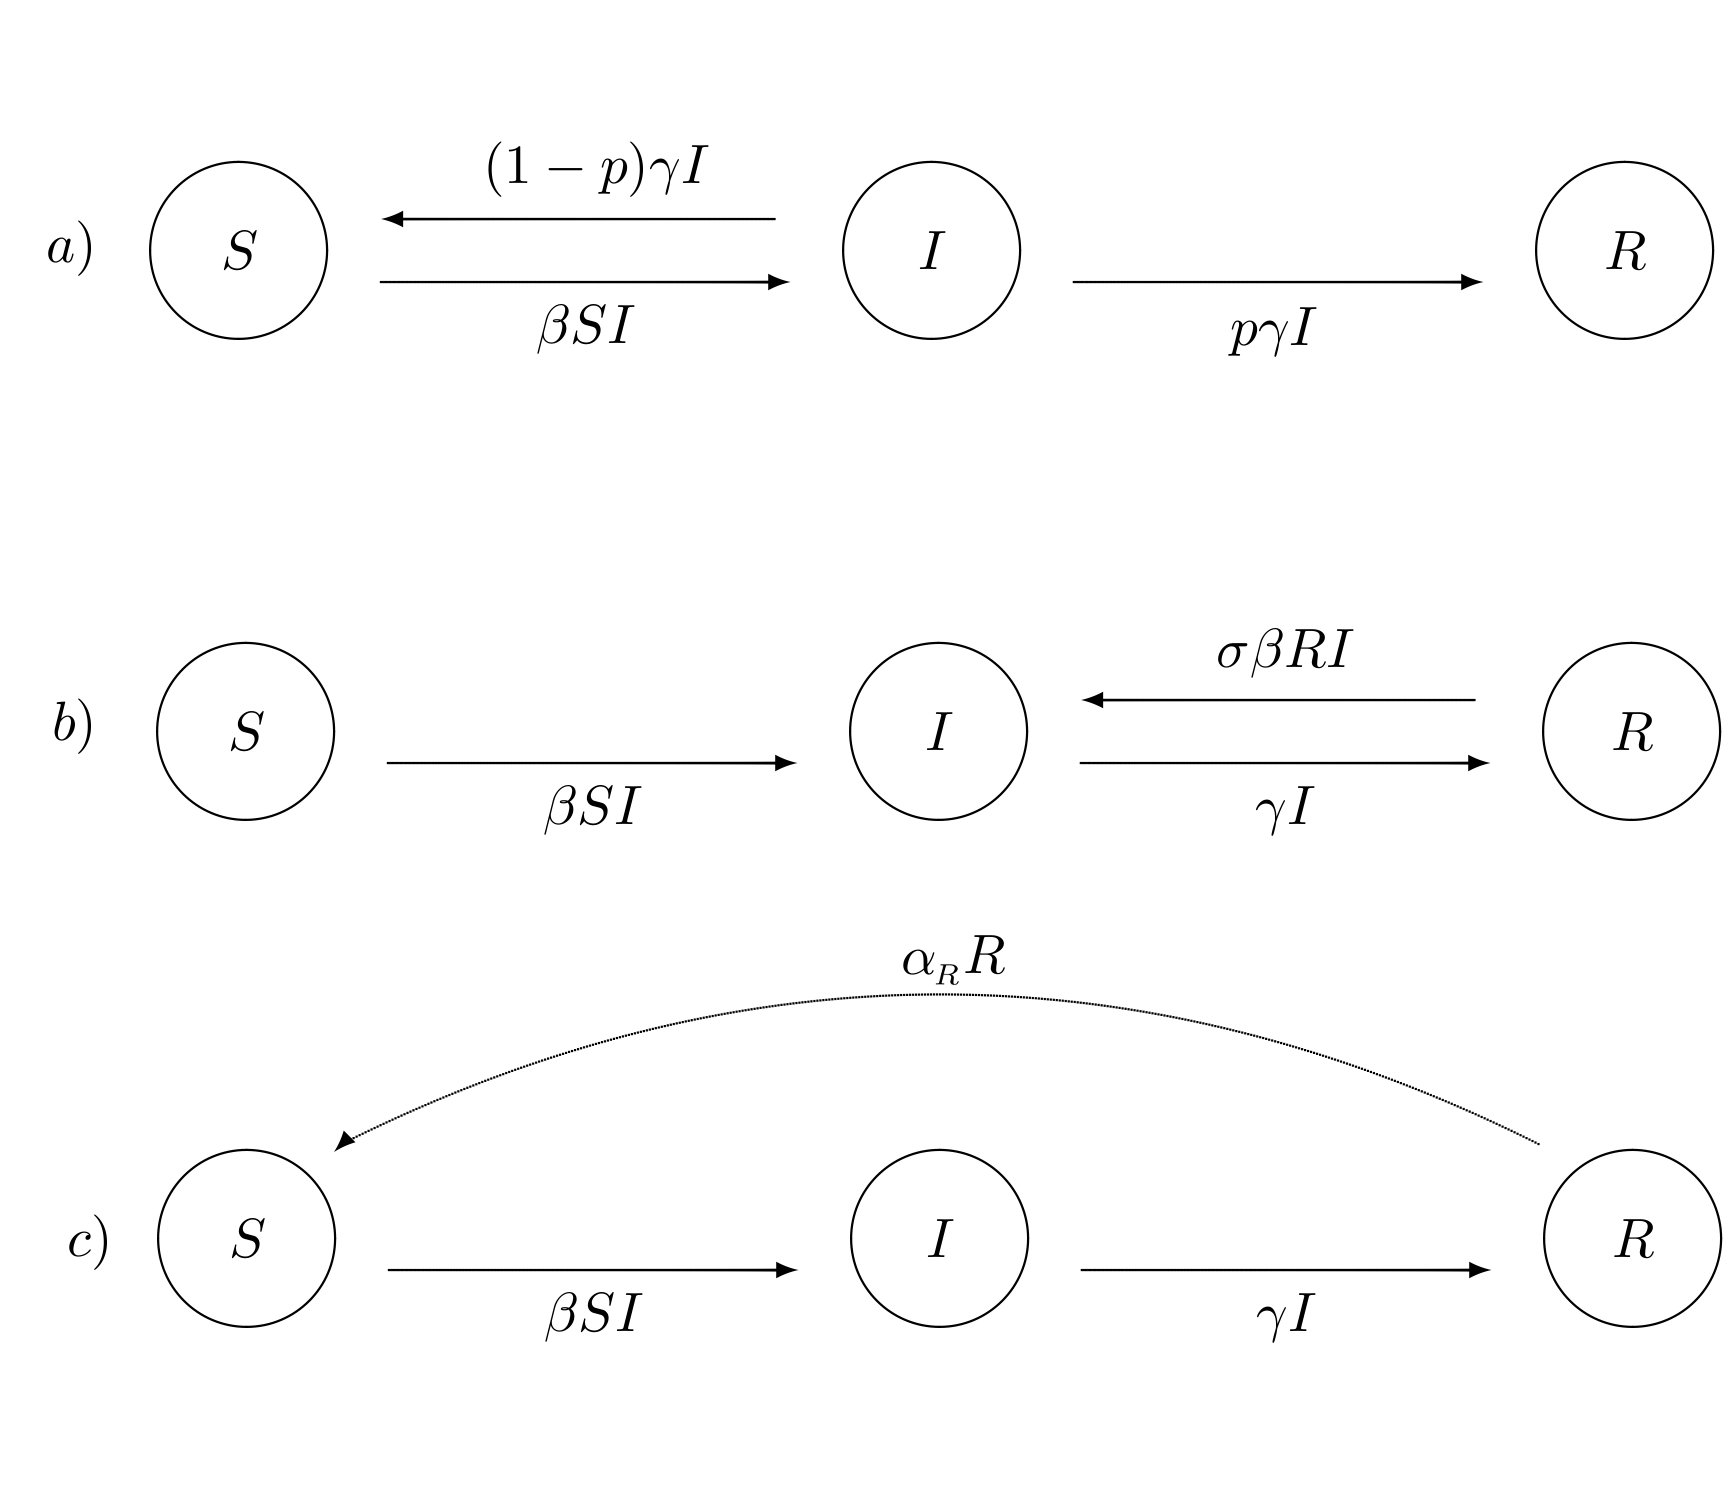
\includegraphics[width=\textwidth]{Figure_Models.jpg}
 \caption{a) All-or-Nothing (AoN) immunity hypothesis \cite{camacho2011explaining}; b) Partially protective immunity (PPI) hypothesis \cite{camacho2011explaining}; c) SIRS model.}
  \label{fig:models}
\end{figure}

\subsection{Global sensitivity analysis for an homogeneous population}
\label{SubSect31}

\par In this SubSection, we consider an individual that behaves equally than the rest of individuals in the population (that is, the population is fully homogeneous). We consider in this section $N=100$ and $\gamma=1$, so that the time unit is the average recovery period of an individual. Our interest is in analysing the probability of this individual suffering exactly $M$ infections for the different values of $M\geq0$, when the different epidemic parameter values change for the SIS and the TPI-SIR models.

\subsubsection{SIS Model: no immunity}

\par In Figure \ref{fig:sis_homogeneous} we focus on the SIS model, where individuals develop no immunity after infection. We plot in Figure \ref{fig:sis_homogeneous} the probability $p_{(N-1,S)}^M-p_{(N-1,S)}^{M+1}$ of individual $A$, initially susceptible, suffering exactly $M$ infections, for $M\in\{0,1,2,3\}$, versus different values of $R_0=\beta N$.
\begin{figure}[h!]
  \centering
 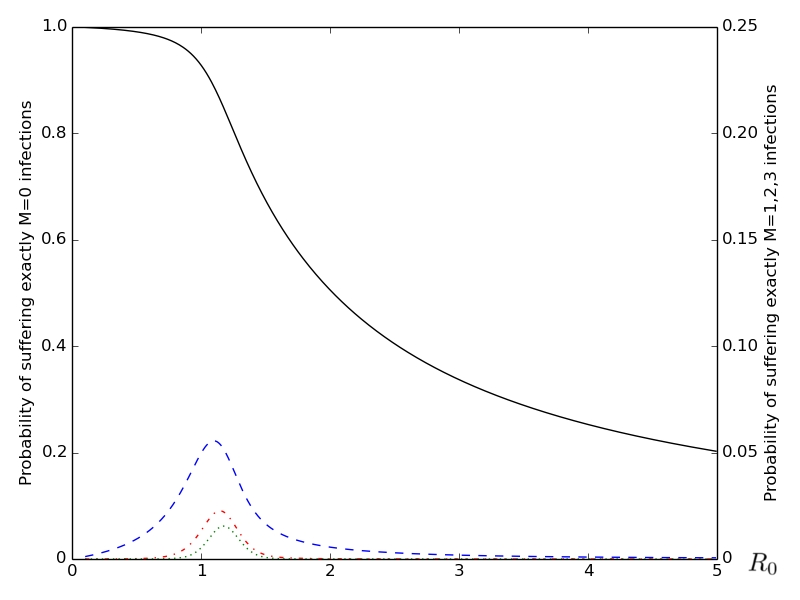
\includegraphics[width=\textwidth]{SIS_Homogeneous.jpg}
 \caption{SIS Model. Probability $p_{(N-1,S)}^M-p_{(N-1,S)}^{M+1}$ of individual $A$, initially susceptible, suffering exactly $M$ infections, for $M\in\{0,1,2,3\}$, versus different values of $R_0=\beta N$. $N=100$, $\gamma=1$. Left y-axis: $M=0$; Right y-axis: $M\in\{1,2,3\}$.}
  \label{fig:sis_homogeneous}
\end{figure}

\par The probability of individual $A$ suffering exactly $0$ infections during the outbreak is $1$ for $R_0=0$, and has a sharp decrease once the value $R_0=1$ is reached, as we could expect. It is interesting to note that the probabilities of individual $A$ suffering exactly $M$ infections, for $M\in\{1,2,3\}$, have maximums for values of $R_0$ slightly larger than $1$. This is directly related to the identification of endemic scenarios. For large values of $R_0>1$, endemicity corresponds to the individual suffering much more than two or three infections. On the other hand, for this individual suffering exactly $1$, exactly $2$ or exactly $3$ infections, very precise values of $R_0$ near but larger than $1$ are required.

\subsubsection{SIRS Model: temporary immunity}

\par In Figure \ref{fig:sirs} our interest is in analysing the SIRS model, where individuals recover susceptibility after a temporary immunity period. We plot in Figure \ref{fig:sirs} probabilities $p_{(N-1,S)}^M-p_{(N-1,S)}^{M+1}$ as in Figure \ref{fig:sis_homogeneous}, while varying the value of $\alpha_R\in\{0.1,0.2,0.5,1.0\}$. We note first that $\alpha_R\rightarrow 0$ represents the $SIR$ model, while $\alpha_R\rightarrow\infty$ corresponds to the $SIS$ model. Thus, for $\alpha_R=1.0$ in Figure \ref{fig:sirs} we already can identify the same behaviours than the ones identified for the SIS model in Figure \ref{fig:sis_homogeneous}. Small value $\alpha_R=0.1$ in Figure \ref{fig:sirs} represents that individuals only recover susceptibility after a long immunity period. This means that, unless we consider a highly infectious disease (large values of $R_0$), individual $A$ will only suffer at most $1$ infection. This can be observed from the maximum corresponding to the probability of suffering exactly $M$ infections, which occurs for a value of $R_0$ slightly larger than $3$, and this curve slowly decreasing for larger values of $R_0$.

\par Shorter immunity periods ({\it e.g.,} $\alpha_R\in\{0.2,0.5\}$) allow the individual to get infected several times, which translates into the maximum for the curve corresponding to $M=1$ occurring closer to $R_0=1$ and decreasing faster after this value. It is also worth to point out that for large values of $R_0$ all the curves for $M\in\{1,2,3\}$ join before reaching values near $0$, which means that for large values of $R_0$, the individual can suffer exactly $1$, exactly $2$ or exactly $3$ infections with equal probability.
\begin{figure}[h!]
  \centering
 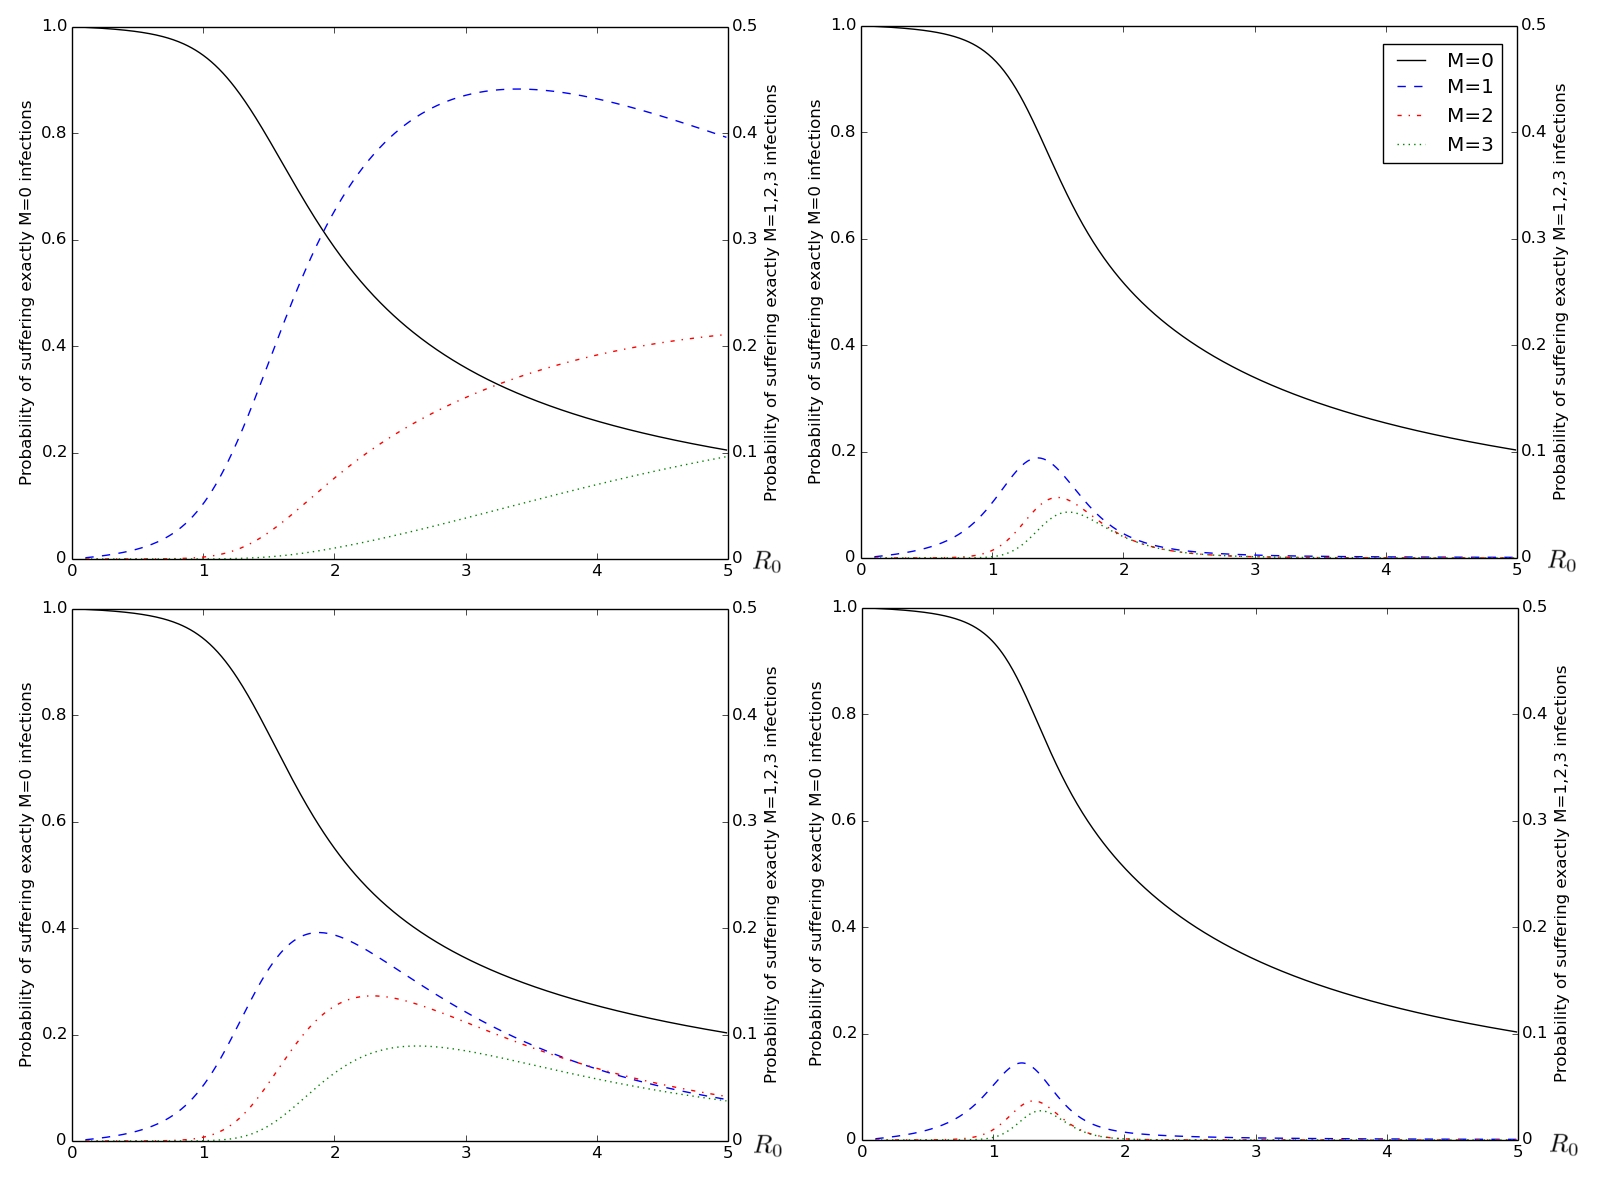
\includegraphics[width=\textwidth]{SIRS.jpg}
 \caption{SIRS Model. Probability $p_{(N-1,S)}^M-p_{(N-1,S)}^{M+1}$ of individual $A$, initially susceptible, suffering exactly $M$ infections, for $M\in\{0,1,2,3\}$, versus different values of $R_0=\beta N$. $\gamma=1$ and $N=100$. Immunity is lost at rate
$\alpha_R=0.1$ ({\it top-left}), $\alpha_R=0.2$ ({\it bottom-left}), $\alpha_R=0.5$ ({\it top-right}) and $\alpha_R=1.0$ ({\it bottom-right}).
Left y-axis: $M=0$; Right y-axis: $M\in\{1,2,3\}$.}
  \label{fig:sirs}
\end{figure}

\subsubsection{PPI Model: partial immunity}

\par In Figure \ref{fig:siri} we consider the PPI model, where individuals get partial immunity after infection, so that recovered individuals can become infected with some probability $\sigma\in(0,1)$. We plot in Figure \ref{fig:siri} the probabilities for the PPI model, while varying $\sigma\in\{0.1,0.2,0.5,1.0\}$. Although the qualitative behaviour of curves in Figures \ref{fig:sirs} and \ref{fig:siri} is similar, we can see that parameter $\sigma$ has a more significant impact than $\alpha_R$ for avoiding re-infection of individuals. That is, temporary immunity allows for the individual to suffer more infections than partial immunity for comparable absolute values of $\alpha_R$ and $\sigma$. This can be observed by looking at curves corresponding to $M\in\{1,2,3\}$ for values $\alpha_R=0.1$ and $\sigma=0.1$ in these Figures, as well as for values $\alpha_R=0.2$ and $\sigma=0.2$.
\begin{figure}[h!]
  \centering
 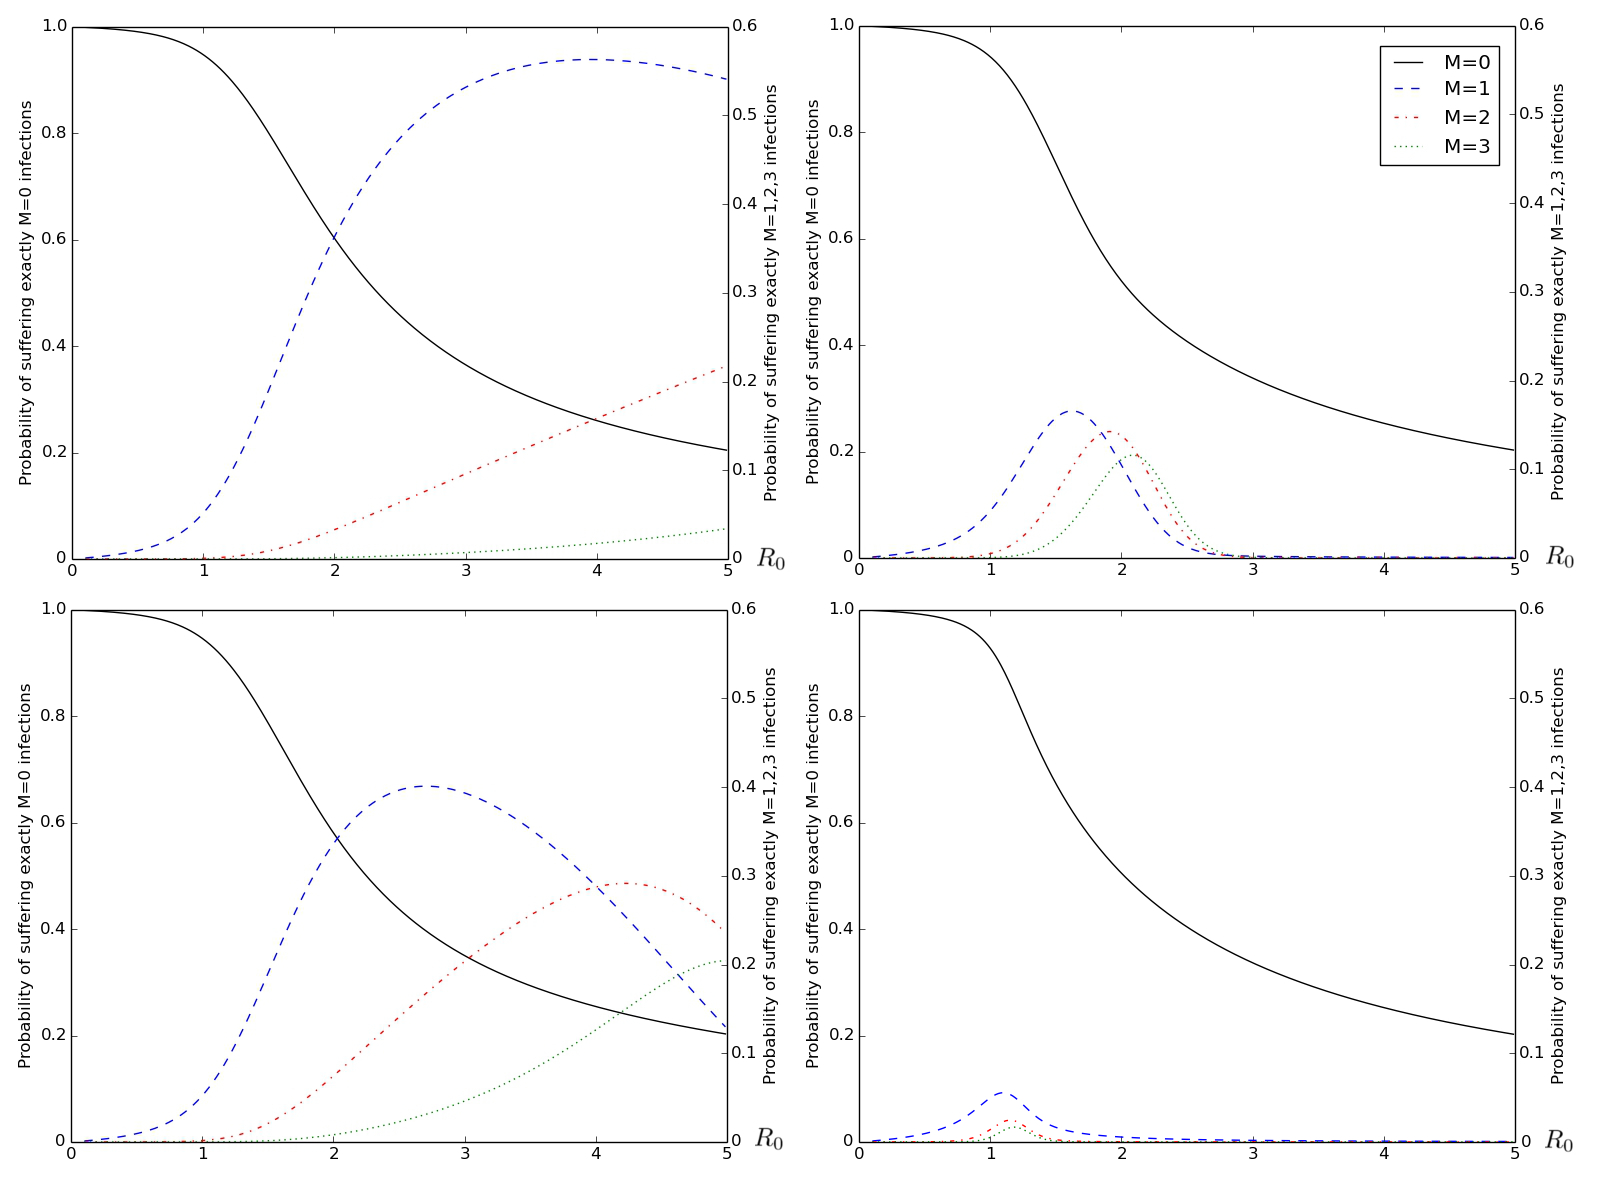
\includegraphics[width=\textwidth]{PPI.jpg}
 \caption{PPI Model. Probability $p_{(N-1,S)}^M-p_{(N-1,S)}^{M+1}$ of individual $A$, initially susceptible, suffering exactly $M$ infections, for $M\in\{0,1,2,3\}$, versus different values of $R_0=\beta N$. $\gamma=1$ and $N=100$.
Partial immunity is represented here by parameter $\sigma=0.1$ ({\it top-left}), $\sigma=0.2$ ({\it bottom-left}), $\sigma=0.5$ ({\it top-right}) and
$\sigma=1.0$ ({\it bottom-right}). Left y-axis: $M=0$; Right y-axis: $M\in\{1,2,3\}$.}
 \label{fig:siri}
\end{figure}

\subsubsection{AoN Model: random immunity}

\par In Figure \ref{fig:aon} we consider the AoN model, where individuals can gain immunity with probability $p$ after infection. In Figure \ref{fig:aon}, we plot probability $p_{(N-1,S)}^M-p_{(N-1,S)}^{M+1}$ of individual $A$, initially susceptible, suffering exactly $M$ infections, for $p\in\{0.1,0.25,0.5,0.75\}$. Asymptotic behaviour of curves in Figure \ref{fig:aon} for $R_0\rightarrow\infty$ is different than the ones observed in the other models considered. In particular, the AoN hypothesis does not yield maximums for each probability plotted in Figure \ref{fig:aon}, so that increasing values of $R_0$ yield threshold values for each probability of suffering exactly $M$ infections, regardless of the value of $M$; see, for example, Figure \ref{fig:aon} {\it top-left}.
\begin{figure}[h!]
  \centering
 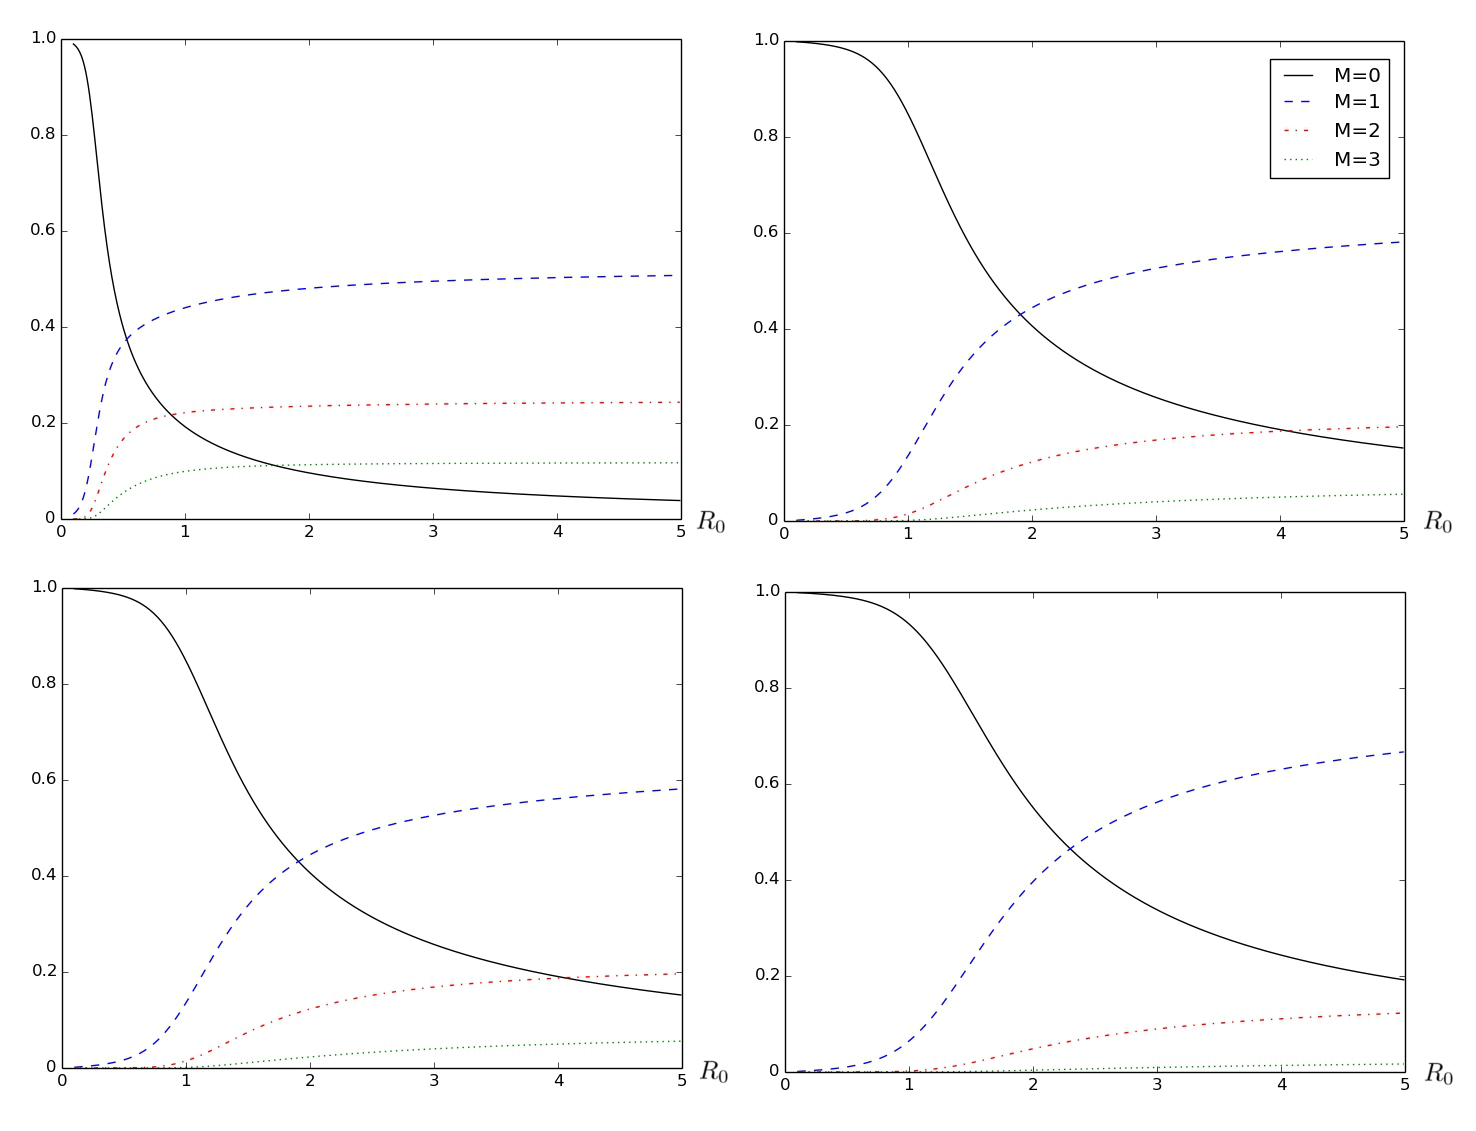
\includegraphics[width=\textwidth]{AoN.jpg}
 \caption{AoN Model. Probability $p_{(N-1,S)}^M-p_{(N-1,S)}^{M+1}$ of individual $A$, initially susceptible, suffering exactly $M$ infections, for $M\in\{0,1,2,3\}$, versus different values of $R_0=\beta N$. $\gamma=1$ and $N=100$. All-or-Nothing probability $p=0.1$ ({\it top-left}), $p=0.25$ ({\it bottom-left}), $p=0.5$ ({\it top-right}) and
$p=0.75$ ({\it bottom-right}). Left y-axis: $M=0$; Right y-axis: $M\in\{1,2,3\}$.}
 \label{fig:aon}
\end{figure}


\subsection{The probabilities of suffering exactly $M$ infections as the likelihood for estimation of parameters: Tristan da Cunha as a case study}
\label{SubSect32}

\par Here, we can fit every model to Tristan da Cunha data and compare. The idea would be to explain how these probabilities can be used as the likelihood when estimating parameters. Moreover, given the large amount of parameters ($\beta$, $\gamma$, $\alpha_R$,...) that we can vary, setting the parameters (at least for the SIRS type models in Figure \ref{fig:4}) by means of this fitting would allow us to keep these parameter values when analysing an heterogeneous individual in SubSection \ref{SubSect33}.

\par We consider... then, we propose the approximated likelihood...
\begin{eqnarray*}
L(\theta;{\underline x}) &=& \dots
\end{eqnarray*}

\begin{table}[h!]
{\small
\centering
\begin{tabular}{|c|c|c|c|c|}
\hline
MLE & SIS & AoN & PPI & SIRS\\
\hline
$\beta$ & & & & \\
\hline
$\gamma$ & & & & \\
\hline
$\sigma$ & $-$ & $-$ & & \\
\hline
$\alpha_R$ & $-$ & & $-$ & \\
\hline
$\alpha_I$ & $-$ & & $-$ & \\
\hline
\end{tabular}
\caption{Maximum likelihood estimates (MLEs)...}
\label{tab:tristan}}
\end{table}


\subsection{Analysis of a especial individual}
\label{SubSect33}

\par In this SubSection, we can plot the histogram of the number of reinfections suffered by individual $A$ (that is, probabilities for $M\in\{0,1,2,3,4\}$ within a histogram) for models SIS, AoN, PPI and SIRS just when parameter values are chosen from Table \ref{tab:tristan}. Now, the question is how the reinfection dynamics of individual A are, when this individual is somehow special. In particular, we consider how these histograms vary when we consider:
\begin{itemize}
 \item Individual $A$ is a {\it super-infectious} individual ($\beta_{A\rightarrow\bullet}=2\beta$),
 \item Individual $A$ is a {\it super-susceptible} individual ($\beta_{\bullet\rightarrow A}=2\beta$),
 \item Individual $A$ is a {\it super-recoverable} individual ($\gamma(A)=2\gamma$).
\end{itemize}

%\par Depending on the results that we get, we might also consider for the TI-SIR, PI-SIR and TPI-SIR models:
%\begin{itemize}
% \item Individual $A$ has better partial immunity ($\sigma(A)=2\sigma$),
% \item Individual $A$ losses immunity faster ($\alpha_R(A)=2\alpha_R$).
%\end{itemize}

\vspace{1cm}

\par\noindent{\large \bf Acknowledgments}\\

\par\noindent This research has been supported by the Medical Research Council through the project MR/N014855/1 (M. L\'opez-Garc\'ia), and by... {\bf Anton Camacho}.\\

\vspace{1cm}

\par\noindent{\large \bf References}
\bibliography{ReinfectionProbability}
\bibliographystyle{plain}

\vspace{1cm}

\par\noindent{\large \bf Appendix A. Probability of suffering at least $M$ infections}\\

\par In this appendix, we show how to generalise our arguments in order to compute the probability of a marked individual $A$ suffering at least $M$
infections, with $M\geq2$. We point out here that, in Section 2, we computed the probability of individual $A$ suffering at least $M=2$ infections
(that is, suffering reinfection). Thus, we generalise our arguments in previous section for any value $M\geq2$, for the SIS and the general TPI-SIR model.\\

\vspace{0.5cm}

\par\noindent{\bf A.1. SIS Model}\\

\par We consider here the extended process ${\cal X}^{ext,M}=\{{\bf X}^{ext,M}(t)=(S^M(t),A^M(t)):\ t\geq0\}$, where we define $A^M(t)$ as the state of
individual $A$ at time $t\geq0$, taking values among $a\in\{S_0,\dots,S_{M-1},I_1,\dots,I_{M-1}\}$. In particular, $A^M(t)=S_j$ (or, alternatively,
$I_j$) represents that individual $A$ is, at current time $t$, susceptible (infected) and suffered exactly $j$ infections up to time $t$. As before, we
can consider that individual $A$ has a different behavior against the disease than the rest of individuals
in the population, by considering specific rates $\gamma(A)$, $\beta_{A\rightarrow\bullet}$ and $\beta_{\bullet\rightarrow A}$.

\par The space of states for our extended process ${\cal X}^{ext,M}$ is given by
\begin{eqnarray*}
 {\cal S}^{ext,M} &=& \left(\{1,\dots,N-1\}\times\{S_0,\dots,S_{M-1},I_1,\dots,I_{M-1}\}\right)\cup\left(\{0\}\times\{I_1,\dots,I_{M-1}\}\right)\\
&&\cup\left(\{N\}\times\{S_0,\dots,S_{M-1}\}\right)\cup\{\Delta^M\},
\end{eqnarray*}
\par\noindent where $\Delta^M$ is an artificial absorbing state representing that individual $A$ suffered, at least, $M$ infections. Transitions
between states in ${\cal S}^{ext,M}$ are given in Table \ref{tab:new1}, and we note that states of the form $(N,a)$ are absorbing states for process ${\cal X}^{ext,M}$
representing the end of the outbreak without individual $A$ suffering $M$ infections.

\begin{table}[h]
\centering
\begin{tabular}{|c|l|l|l|}
\hline
Event & Original state & Destination state & Rate\\
\hline
Recovery of & $(m,S_j)$, $m\geq1$ & $(m+1,S_j)$ & $\gamma(N-m)$\\
an infective & $(m,I_j)$, $j\geq1$ & $(m+1,S_j)$ & $\gamma(A)$\\
individual & $(m,I_j)$, $m\leq N-2$, $j\geq1$ & $(m+1,I_j)$ & $\gamma(N-m-1)$\\
\hline
Infection of & $(m,S_j)$, $m\geq1$, $j\leq M-2$ & $(m-1,I_{j+1})$ & $\beta_{\bullet\rightarrow A}(N-m)$\\
a susceptible & $(m,S_{M-1})$, $m\geq1$ & $\Delta^M$ & $\beta_{\bullet\rightarrow A}(N-m)$\\
individual & $(m,S_j)$, $m\geq2$ & $(m-1,S_j)$ & $\beta(m-1)(N-m)$\\
 & $(m,I_j)$, $j\geq1$ & $(m-1,I_j)$ & $\beta m(N-m-1)+\beta_{A\rightarrow\bullet}m$\\
\hline
\end{tabular}
\caption{Transitions among states in ${\cal S}^{ext,M}$, for $0\leq m\leq N-1$, $0\leq j\leq M-1$.}
\label{tab:new1}
\end{table}

\par We define $p^M_{(m,a)}$ as the probability of individual $A$ suffering at least $M$ infections, given the initial state of the process $(m,a)\in{\cal S}^{ext,M}$,
with trivial probabilities $p^M_{\Delta^M}=1$, $p^M_{(N,S_j)}=0$ for all $0\leq j\leq M-1$. These probabilities satisfy, for $0\leq m\leq N-1$, $0\leq j\leq M-1$, the equations
\vspace{1cm}
\begin{eqnarray*}
 \theta_{(m,S)}p^M_{(m,S_j)} &=& \beta(m-1)(N-m)p^M_{(m-1,S_j)}+\beta_{\bullet\rightarrow A}(N-m)(1_{j=M-1}p^M_{\Delta^M}\\
&&+1_{j<M-1}p^M_{(m-1,I_{j+1})})+\gamma(N-m)p^M_{(m+1,S_j)},\quad m\geq1,\quad (Equation\ (E.S_j))\\
\theta_{(m,I)}p^M_{(m,I_j)} &=& \left(\beta m(N-m-1)+\beta_{A\rightarrow\bullet}m\right)p^M_{(m-1,I_j)}+\gamma(N-m-1)p^M_{(m+1,I_j)}\\
&&+\gamma(A)p^M_{(m+1,S_j)},\quad j\geq 1,\quad (Equation\ (E.I_j))
\end{eqnarray*}
\par\noindent with $\theta_{(m,S)}$ and $\theta_{(m,I)}$ defined in Section 2, and $1_{\cal B}$ a boolean function taking value $1$ if condition ${\cal B}$ is verified, and $0$ otherwise. These equations are directly related to the transitions diagram of ${\cal X}^{ext,M}$, given in Figure \ref{fig:3new}.

\begin{figure}[h!]
\centering
 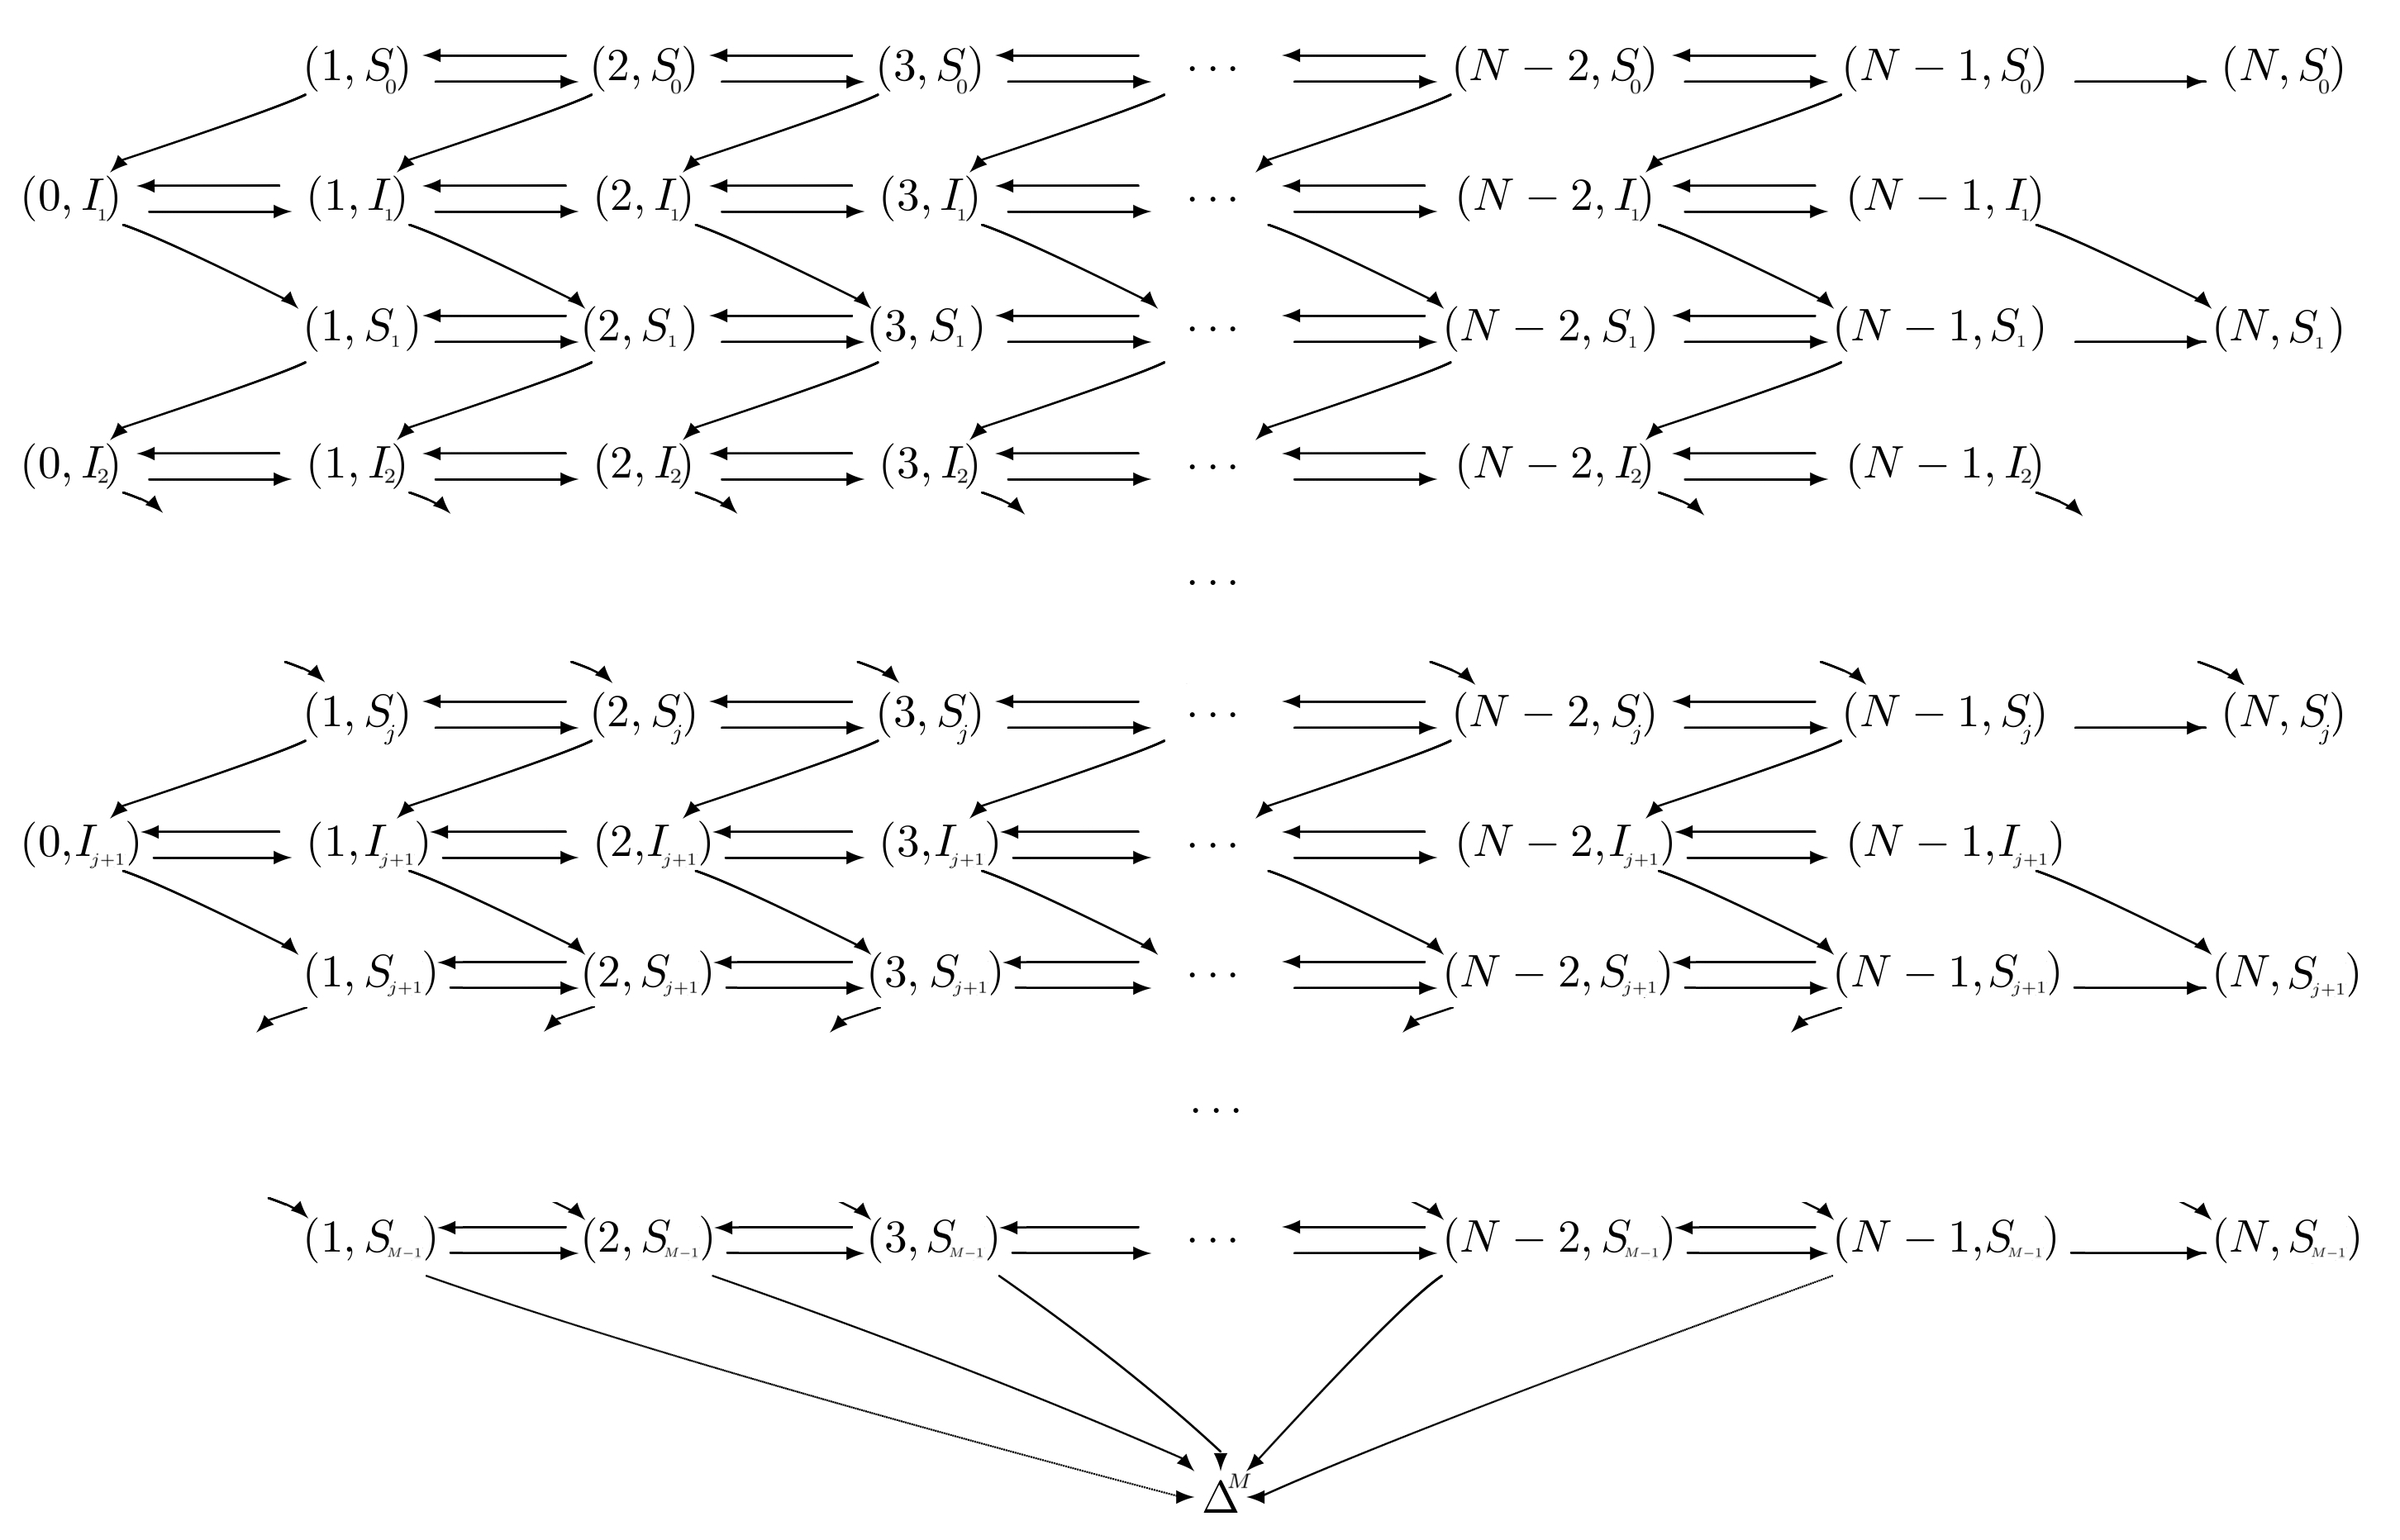
\includegraphics[width=\textwidth]{Figure3_new.jpg}
\caption{Transitions diagram for process ${\cal X}^{ext,M}$.}
\label{fig:3new}
\end{figure}

\par This diagram also gives some clue on how to iteratively solve the system of equations given by Eqs. $(E.S_j)-(E.I_j)$. In particular, we can start
solving Equations $(E.S_{M-1})$ for $1\leq m\leq N$ and, once probabilities $p^M_{(m,S_{M-1})}$ are in hand, Equations $(E.I_{M-1})$ can be solved, obtaining
probabilities $p^M_{(m,I_{M-1})}$ for $0\leq m\leq N-1$. Then, we can continue working in an algorithmic fashion solving Eqs. $(E.I_j)$ after Eqs.
$(E.S_j)$. In particular, if we develop {\bf Algorithms} $S_j$ and $I_j$ (following the same arguments than in Section 2), probabilities of interest
are computed as follows:

\begin{description}
  \item \it Run Algorithm $S_{M-1}$;
  \item \it For $j=M-2,\dots,0$:
  \item $~$\hspace{0.5cm} \it Run Algorithm $I_{j+1}$;
  \item $~$\hspace{0.5cm} \it Run Algorithm $S_{j}$;
\end{description}

\par\noindent with {\bf Algorithms $S_j$} and $I_j$ described below.\\

\par \noindent{\bf Algorithm $S_j$, $0\leq j\leq M-1$}
\begin{description}
  \item $g_{(N-1,S_j)} ~=~ \frac{\beta_{\bullet\rightarrow A}}{\theta_{(N-1,S)}}\left(1_{j=M-1}+1_{j<M-1}p^M_{(N-2,I_{j+1})}\right)$;
  \item \it For $m=N-2,\dots,1$:
  \item $~$\hspace{0.5cm} $g_{(m,S_j)} ~=~ \frac{\beta_{\bullet\rightarrow A}(N-m)}{\theta_{(m,S)}}\left(1_{j=M-1}+1_{j<M-1}p^M_{(m-1,I_{j+1})}\right)+\frac{\gamma(N-m)}{\theta_{(m,S)}}h_{(m+1,S)}^{-1}g_{(m+1,S_j)}$;
  \item $p^M_{(1,S_j)} ~=~ h_{(1,S)}^{-1}g_{(1,S_j)}$;
  \item \it For $m=2,\dots,N-1$:
  \item $~$\hspace{0.5cm} $p^M_{(m,S_j)} ~=~ h_{(m,S)}^{-1}\left(f_{(m,S)}p^M_{(m-1,S_j)}+g_{(m,S_j)}\right)$;
\end{description}

\vspace{0.5cm}
\par \noindent{\bf Algorithm $I_j$, $1\leq j\leq M-1$}
\begin{description}
  \item $g_{(N-1,I_j)} ~=~ \frac{\gamma(A)}{\theta_{(N-1,I)}}p^M_{(N,S_{j})}$;
  \item \it For $m=N-2,\dots,0$:
  \item $~$\hspace{0.5cm} $g_{(m,I_j)} ~=~ \frac{\gamma(A)}{\theta_{(m,I)}}p^M_{(m+1,S_j)}+\frac{\gamma(N-m-1)}{\theta_{(m,I)}}h_{(m+1,I)}^{-1}g_{(m+1,I_j)}$;
  \item $p^M_{(0,I_j)} ~=~ h_{(0,I)}^{-1}g_{(0,I_j)}$;
  \item \it For $m=1,\dots,N-1$:
  \item $~$\hspace{0.5cm} $p^M_{(m,I_j)} ~=~ h_{(m,I)}^{-1}\left(f_{(m,I)}p^M_{(m-1,I_j)}+g_{(m,I_j)}\right)$;
\end{description}

\par\noindent We note here that quantities $h_{(m,S)}$, $f_{(m,S)}$, $h_{(m,I)}$ and $f_{(m,I)}$ are the ones computed in {\bf Algorithm 1}, since they do not depend
on the value of $j$. Finally, it is worth to point out that, once probabilities $p^M_{(m,a)}$ are in hand for different values of $M$, the probability
of individual $A$ suffering exactly $M$ infections given the initial state $(m,a)$ is given by $p^M_{(m,a)}-p^{M+1}_{(m,a)}$.\\

\vspace{0.5cm}

\par\noindent{\bf A.2. TPI-SIR model}\\

\par We proceed here as before and define the extended process ${\cal \tilde X}^{ext,M}=\{{\bf \tilde X}^{ext,M}(t)=({\tilde S}^M(t),{\tilde I}^M(t),{\tilde A}^M(t)):\ t\geq0\}$ where
${\tilde A}^M(t)$ takes values among $a\in\{S_0,\dots,S_{M-1},I_1,\dots,I_{M-1},\linebreak R_1,\dots,R_{M-1}\}$. ${\cal \tilde X}^{ext,M}$ is defined over the
space of states
\begin{eqnarray*}
 {\cal \tilde S}^{ext,M} &=& \left({\cal \tilde S}^{ext,M}(S)\times\{S_0,\dots,S_{M-1}\}\right)\cup\left({\cal \tilde S}^{ext,M}(I)\times\{I_1,\dots,I_{M-1}\}\right)\\
 &&\cup\left({\cal \tilde S}^{ext,M}(R)\times\{R_1,\dots,R_{M-1}\}\right)\cup\{{\tilde \Delta}^M\},
\end{eqnarray*}
\par\noindent where ${\tilde \Delta}^M$ is the artificial absorbing state representing that individual $A$ suffered at least $M$ infections, and
where
\begin{eqnarray*}
 {\cal \tilde S}^{ext,M}(S) &=& \{(m,n)\in\mathbb{N}_0^2:\ m>0,\ m+n\leq N\},\\
{\cal \tilde S}^{ext,M}(I) &=& \{(m,n)\in\mathbb{N}_0^2:\ n>0,\ m+n\leq N\},\\
{\cal \tilde S}^{ext,M}(R) &=& \{(m,n)\in\mathbb{N}_0^2:\ m+n<N\},
\end{eqnarray*}

\par\noindent relate to the numbers of susceptible and infective individuals when individual $A$ is susceptible, infective or recovered, respectively.
Possible transitions among states in our extended process are given in Table \ref{tab:2new}, where states of the form $(m,0,a)$ are considered as
absorbing states, since they represent the situation where no infective individuals remain in the population.

\begin{table}[h]
{\small
\centering
\begin{tabular}{|c|l|l|l|}
\hline
Event & Original state & Destination state & Rate\\
\hline
Recovery & $(m,n,S_j)$, $m\geq1$, & $(m,n-1,S_j)$ & $\gamma n$\\
of an & $(m,n,I_j)$,  $n\geq2$, $j\geq1$ & $(m,n-1,I_j)$ & $\gamma(n-1)$\\
infective & $(m,n,I_j)$, $j\geq1$ & $(m,n-1,R_j)$ & $\gamma(A)$\\
individual & $(m,n,R_j)$, $m+n<N$, $j\geq1$ & $(m,n-1,R_j)$ & $\gamma n$\\
\hline
Infection & $(m,n,S_{M-1})$, $m\geq1$ & ${\tilde \Delta}^M$ & $\beta_{\bullet\rightarrow A}n$\\
of a & $(m,n,S_j)$, $m\geq2$ & $(m-1,n+1,S_j)$ & $\beta(m-1)n$\\
susceptible & $(m,n,S_j)$, $m\geq1$, $j\leq M-2$ & $(m-1,n+1,I_{j+1})$ & $\beta_{\bullet\rightarrow A}n$\\
individual & $(m,n,I_j)$, $m\geq1$, $j\geq1$ & $(m-1,n+1,I_j)$ & $\beta m(n-1)+\beta_{A\rightarrow\bullet}m$\\
 & $(m,n,R_j)$, $m\geq1,\ m+n<N$, $j\geq1$ & $(m-1,n+1,R_j)$ & $\beta mn$\\
\hline
Infection & $(m,n,S_j)$, $m\geq1,\ m+n<N$, $j\geq1$ & $(m,n+1,S_j)$ & $\sigma\beta n(N-m-n)$\\
of a & $(m,n,I_j)$, $m+n<N$, $j\geq1$ & $(m,n+1,I_j)$ & $\sigma\beta(n-1)(N-m-n)$\\
recovered & & & $+\sigma\beta_{A\rightarrow\bullet}(N-m-n)$\\
individual & $(m,n,R_j)$, $m+n<N-1$, $j\geq1$ & $(m,n+1,R_j)$ & $\sigma\beta n(N-m-n-1)$\\
 & $(m,n,R_j)$, $m+n<N$, $1\leq j\leq M-2$ & $(m,n+1,I_{j+1})$ & $\sigma(A)\beta_{\bullet\rightarrow A} n$\\
 & $(m,n,R_{M-1})$, $m+n<N$ & ${\tilde \Delta}^{M}$ & $\sigma(A)\beta_{\bullet\rightarrow A} n$\\
\hline
Immunity & $(m,n,S_j)$, $m\geq1$ & $(m+1,n-1,S_j)$ & $\alpha_I n$\\
loss of an & $(m,n,I_j)$, $n\geq2$, $j\geq1$ & $(m+1,n-1,I_j)$ & $\alpha_I(n-1)$\\
infective & $(m,n,I_j)$, $j\geq1$ & $(m+1,n-1,S_j)$ & $\alpha_I(A)$\\
individual & $(m,n,R_j)$, $m+n<N$, $j\geq1$ & $(m+1,n-1,R_j)$ & $\alpha_I n$\\
\hline
Immunity & $(m,n,S_j)$, $m\geq1,\ m+n<N$ & $(m+1,n,S_j)$ & $\alpha_R (N-m-n)$\\
loss of a & $(m,n,I_j)$, $m+n<N$, $j\geq1$ & $(m+1,n,I_j)$ & $\alpha_R (N-m-n)$\\
recovered & $(m,n,R_j)$, $m+n<N-1$, $j\geq1$ & $(m+1,n,R_j)$ & $\alpha_R (N-m-n-1)$\\
individual & $(m,n,R_j)$, $m+n<N$, $j\geq1$ & $(m+1,n,S_j)$ & $\alpha_R(A)$\\
\hline
\end{tabular}
\caption{Transitions among states in ${\cal \tilde S}^{ext,M}$, for $m\geq0$, $n\geq1$, $m+n\leq N$, and $0\leq j\leq M-1$.}
\label{tab:2new}}
\end{table}

\par If we define
\begin{eqnarray*}
 p^M_{(m,n,a)} &=& \hbox{\it ``probability of individual $A$ suffering at least $M$ infections, given}\\
&& \hbox{\it the initial state of the process $(m,n,a)\in{\cal \tilde S}^{ext,M}$''},
\end{eqnarray*}
\par\noindent these probabilities satisfy the following equations, for $m\geq0$, $n\geq1$, $m+n\leq N$ and $0\leq j\leq M-1$,
\begin{eqnarray*}
 \theta_{(m,n,S)}p^M_{(m,n,S_j)} &=& \beta(m-1)np^M_{(m-1,n+1,S_j)}+\beta_{\bullet\rightarrow A}n\left(1_{j=M-1}p^M_{{\tilde \Delta}^M}+1_{j<M-1}p^M_{(m-1,n+1,I_{j+1})}\right)\\
&&+\gamma np^M_{(m,n-1,S_j)}+\alpha_I np^M_{(m+1,n-1,S_j)}+\alpha_R(N-m-n)p^M_{(m+1,n,S_j)}\\
&&+\sigma\beta n(N-m-n)p^M_{(m,n+1,S_j)},\quad m\geq1,\ (Equation\ ({\tilde E}.S_j))\\
 \theta_{(m,n,I)}p^M_{(m,n,I_j)} &=& \left(\beta m(n-1)+\beta_{A\rightarrow\bullet}m\right)p^M_{(m-1,n+1,I_j)}+\gamma(n-1)p^M_{(m,n-1,I_j)}\\
&&+\gamma(A)p^M_{(m,n-1,R_j)}+\alpha_I(n-1)p^M_{(m+1,n-1,I_j)}+\alpha_I(A)p^M_{(m+1,n-1,S_j)}\\
&&+\left(\sigma\beta(n-1)(N-m-n)+\sigma\beta_{A\rightarrow\bullet}(N-m-n)\right)p^M_{(m,n+1,I_j)}\\
&& +\alpha_R(N-m-n)p^M_{(m+1,n,I_j)},\quad j\geq1,\quad (Equation\ ({\tilde E}.I_j))\\
 \theta_{(m,n,R)}p^M_{(m,n,R_j)} &=& \beta mnp^M_{(m-1,n+1,R_j)}+\gamma np^M_{(m,n-1,R_j)}+\alpha_I np^M_{(m+1,n-1,R_j)}\\
&&+\alpha_R(N-m-n-1)p^M_{(m+1,n,R_j)}+\alpha_R(A)p^M_{(m+1,n,S_j)}\\
&&+\sigma\beta n(N-m-n-1)p^M_{(m,n+1,R_j)}+\sigma(A)\beta_{\bullet\rightarrow A}n\left(1_{j=M-1}p^M_{{\tilde \Delta}^M}\right.\\
&&\left.+1_{j<M-1}p^M_{(m,n+1,I_{j+1})}\right),\quad m+n<N,\ j\geq1,\quad (Equation\ ({\tilde E}.R_j))
\end{eqnarray*}
\par\noindent with $\theta_{(m,n,S)}$, $\theta_{(m,n,I)}$ and $\theta_{(m,n,R)}$ defined in Section 2, and boundary conditions
$p^M_{{\tilde \Delta}^M}=1$, $p_{(m,0,S_j)}=p_{(m,0,R_j)}=0$ for any $m$ and $j$. These equations can be solved one after the other following the diagram
in Figure \ref{fig:diag}. This iterative procedure can be carried out by means of implementing a series of algorithms ({\bf Algorithms} ${\tilde S}_{j}$,
${\tilde I}_{j}$ and ${\tilde R}_{j}$). In particular:
\begin{description}
  \item \it Run Algorithm ${\tilde S}_{M-1}$;
  \item \it For $j=M-2,\dots,0$:
  \item $~$\hspace{0.5cm} \it Run Algorithm ${\tilde R}_{j+1}$;
  \item $~$\hspace{0.5cm} \it Run Algorithm ${\tilde I}_{j+1}$;
  \item $~$\hspace{0.5cm} \it Run Algorithm ${\tilde S}_{j}$;
\end{description}

\begin{figure}
\centering
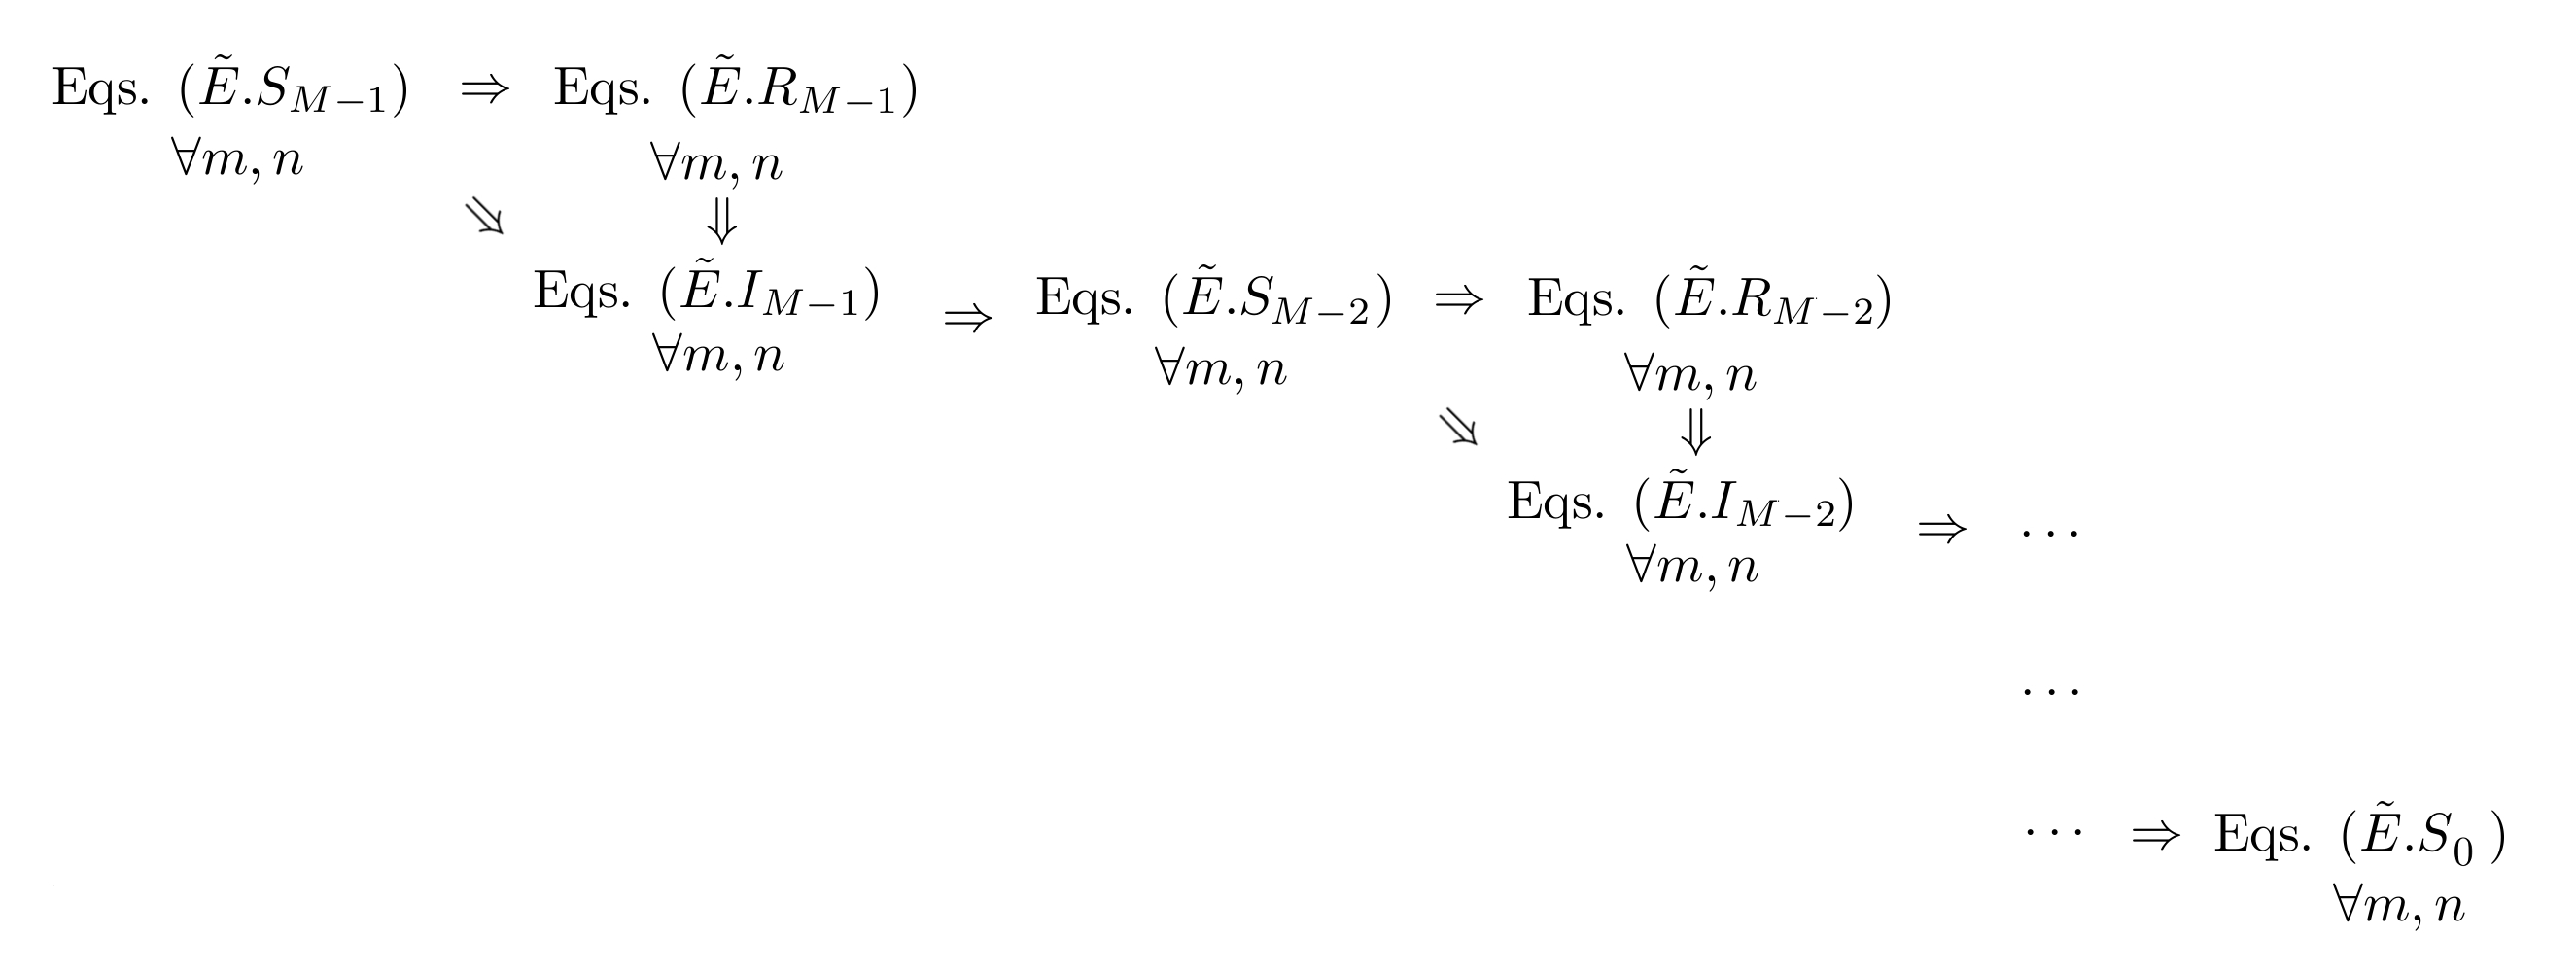
\includegraphics[width=\textwidth]{FigureSolutionNew.jpg}
\caption{Diagram for solving Eqs. $({\tilde E}.S_j)-({\tilde E}.I_j)-({\tilde E}.R_j)$ for all values of $j$.}
\label{fig:diag}
\end{figure}

\vspace{0.5cm}
\par \noindent{\bf Algorithm ${\tilde S_j}$}
\begin{description}
  \item ${\bf J}^M_2(S_j) ~=~ {\bf b}^M_2(S_j)$;
  \item \it For $k=3,\dots,N$:
  \item $~$\hspace{0.5cm} ${\bf J}^M_k(S_j) ~=~ {\bf A}_{k,k-1}(S){\bf H}_{k-1}(S)^{-1}{\bf J}^M_{k-1}(S_j)+{\bf b}^M_k(S_j)$;
  \item ${\bf p}^M_N(S_j) ~=~ {\bf H}_N(S)^{-1}{\bf J}^M_N(S_j)$;
  \item \it For $k=N-1,\dots,2$:
  \item $~$\hspace{0.5cm} ${\bf p}^M_k(S_j) ~=~ {\bf H}_k(S)^{-1}\left({\bf A}_{k,k+1}(S){\bf p}^M_{k+1}(S_j)+{\bf J}^M_k(S_j)\right)$;
\end{description}

\vspace{0.5cm}
\par \noindent{\bf Algorithm ${\tilde R_j}$}
\begin{description}
  \item ${\bf J}^M_1(R_j) ~=~ {\bf b}^M_1(R_j)$;
  \item \it For $k=2,\dots,N-1$:
  \item $~$\hspace{0.5cm} ${\bf J}^M_k(R_j) ~=~ {\bf A}_{k,k-1}(R){\bf H}_{k-1}(R)^{-1}{\bf J}^M_{k-1}(R_j)+{\bf b}^M_k(R_j)$;
  \item ${\bf p}^M_{N-1}(R_j) ~=~ {\bf H}_{N-1}(R)^{-1}{\bf J}^M_{N-1}(R_j)$;
  \item \it For $k=N-2,\dots,1$:
  \item $~$\hspace{0.5cm} ${\bf p}^M_k(R_j) ~=~ {\bf H}_k(R)^{-1}\left({\bf A}_{k,k+1}(R){\bf p}^M_{k+1}(R_j)+{\bf J}^M_k(R_j)\right)$;
\end{description}

\vspace{0.5cm}
\par \noindent{\bf Algorithm ${\tilde I_j}$}
\begin{description}
  \item ${\bf J}^M_1(I_j) ~=~ {\bf b}^M_1(I_j)$;
  \item \it For $k=2,\dots,N-1$:
  \item $~$\hspace{0.5cm} ${\bf J}^M_k(I_j) ~=~ {\bf A}_{k,k-1}(I){\bf H}_{k-1}(I)^{-1}{\bf J}^M_{k-1}(I_j)+{\bf b}^M_k(I_j)$;
  \item ${\bf p}^M_{N-1}(I_j) ~=~ {\bf H}_{N-1}(I)^{-1}{\bf J}^M_{N-1}(I_j)$;
  \item \it For $k=N-2,\dots,1$:
  \item $~$\hspace{0.5cm} ${\bf p}^M_k(I_j) ~=~ {\bf H}_k(I)^{-1}\left({\bf A}_{k,k+1}(I){\bf p}^M_{k+1}(I_j)+{\bf J}^M_k(I_j)\right)$;
\end{description}

\par\noindent We note that:
\begin{itemize}
  \item Matrices ${\bf A}_{k,k'}(S)$, ${\bf A}_{k,k'}(I)$, ${\bf A}_{k,k'}(R)$, ${\bf H}_k(S)$, ${\bf H}_k(I)$ and ${\bf H}_k(R)$ are defined in Section 2.
  \item Probability vectors ${\bf p}^M_k(S_j)$, ${\bf p}^M_k(I_j)$ and ${\bf p}^M_k(R_j)$ contain the desired probabilities $p^M_{(m,n,a)}$, and are structured in a similar
fashion than vectors ${\bf p}_k(S)$, ${\bf p}_k(I)$ and ${\bf p}_k(R)$ in Section 2.
  \item Vectors ${\bf b}^M_k(\cdot)$ are given as follows
\begin{eqnarray*}
 {\bf b}^M_k(S_j) & = & \left(\begin{array}{c}
               \frac{\beta_{\bullet\rightarrow A}}{\theta_{(k-1,1,S)}}\left(1_{j=M-1}+1_{j<M-1}p^M_{(k-2,2,I_{j+1})}\right)\\
\frac{\beta_{\bullet\rightarrow A}2}{\theta_{(k-2,2,S)}}\left(1_{j=M-1}+1_{j<M-1}p^M_{(k-3,3,I_{j+1})}\right)\\
\vdots\\
\frac{\beta_{\bullet\rightarrow A}(k-1)}{\theta_{(1,k-1,S)}}\left(1_{j=M-1}+1_{j<M-1}p^M_{(0,k,I_{j+1})}\right)\\
                         \end{array}\right),\\
{\bf b}^M_k(I_j) & = & \left(\begin{array}{c}
               0\\
\frac{\gamma(A)p^M_{(k-2,1,R_j)}+\alpha_I(A)p^M_{(k-1,1,S_j)}}{\theta_{(k-2,2,I)}}\\
\vdots\\
\frac{\gamma(A)p^M_{(0,k-1,R_j)}+\alpha_I(A)p^M_{(1,k-1,S_j)}}{\theta_{(0,k,I)}}
                         \end{array}\right),\\
{\bf b}^M_k(R_j) & = & \left(\begin{array}{c}
\frac{\alpha_R(A)p^M_{(k,1,S_j)}+\sigma(A)\beta_{\bullet\rightarrow A}\left(1_{j=M-1}+1_{j<M-1}p^M_{(k-1,2,I_{j+1})}\right)}{\theta_{(k-1,1,R)}}\\
\frac{\alpha_R(A)p^M_{(k-1,2,S_j)}+2\sigma(A)\beta_{\bullet\rightarrow A}\left(1_{j=M-1}+1_{j<M-1}p^M_{(k-2,3,I_{j+1})}\right)}{\theta_{(k-2,2,R)}}\\
\vdots\\
\frac{\alpha_R(A)p^M_{(1,k,S_j)}+k\sigma(A)\beta_{\bullet\rightarrow A}\left(1_{j=M-1}+1_{j<M-1}p^M_{(0,k+1,I_{j+1})}\right)}{\theta_{(0,k,R)}}
                         \end{array}\right).
\end{eqnarray*}

\end{itemize}

\par\noindent Finally, once probabilities $p^M_{(m,n,a)}$ are in hand for different values of $M$, the probability of individual $A$ suffering exactly
$M$ infections is given by $p^M_{(m,n,a)}-p^{M+1}_{(m,n,a)}$.\\

\vspace{0.5cm}

\par\noindent{\bf A.3. The number of individuals suffering at least $M$ infections}\\

\par We finally point out here that, for a completely homogeneous population and the SIS model (same arguments apply for the general TPI-SIR model), if the individual starting the infection is randomly chosen among individuals in the population, it is clear that
\begin{eqnarray*}
p^M &=& \mathbb{P}(\hbox{\it $A$ suffering at least $M$ infections}) \ = \ p^M_{(m-1,S_0)}\frac{N-1}{N}+p^M_{(m-1,I_1)}\frac{1}{N}.
\end{eqnarray*}
\par\noindent Then, if we are interested in the random variable
\begin{eqnarray*}
 Y^M &=& \hbox{\it ``Number of individuals in the population suffering at least $M$ infections''},
\end{eqnarray*}
\par\noindent it is clear that
\begin{eqnarray*}
 p^M &=& \sum\limits_{y=0}^N\mathbb{P}(\hbox{\it $A$ suffering at least $M$ infections $|$ $Y^M=y$})\mathbb{P}(Y^M=y)
\end{eqnarray*}
\par\noindent and, since all the individuals are {\it symmetric}, we get
\begin{eqnarray*}
 p^M &=& \sum\limits_{y=0}^N\frac{y}{N}\mathbb{P}(Y^M=y) \ = \ \frac{E[Y^M]}{N}
\end{eqnarray*}
\par\noindent Thus, once probabilities $p^M_{(m,a)}$ are in hand, we can easily obtain $E[Y^M]$ as
\begin{eqnarray*}
E[Y^M] &=& (N-1)p^M_{(m-1,S_0)}+p^M_{(m-1,I_1)},
\end{eqnarray*}
\par\noindent while the probability mass function of $Y^M$ could also be computed by following first-step arguments, which is out of the scope of
this paper.

\end{document}
